

\section{Abstract Theory}

\section{Analysis of the Stokes Equations}
The strong form of the Stokes problem with which we begin is as follows:

\begin{align}
- \mu \Delta \NVRvect{u} + \NVRgrad p &= \NVRvect{f} & \text{ in } \Omega, \label{NVR:eq:strongfirst1} \\
\NVRdiv \NVRvect{u} &= 0 & \text{ in } \Omega, \\
\NVRvect{u} &= \NVRvect{g_{D}} & \text{ on } \partial\Omega,\label{NVR:eq:stronglast1}
\end{align}
where $\Omega \subset \mathbb{R}^{2}$, $\mu$ is viscosity, $\NVRtensor{\epsilon}=\NVRgrad^{\text{sym}} \NVRvect{u}$ is strain, $p$ is pressure, $u$ velocity, and $\NVRvect{f}$ a vector forcing function.

For DPG, we require a first-order system.  We introduce $\NVRtensor{\sigma}=\mu \NVRgrad \NVRvect{u}$:
\begin{align}
\frac{1}{\mu} \NVRtensor{\sigma} - \NVRgrad \NVRvect{u} &= 0 \\
- \mu \NVRdiv \NVRtensor{\sigma} + \NVRgrad p &= \NVRvect{f} & \text{ in } \Omega, \label{NVR:eq:strongfirst2} \\
\NVRdiv \NVRvect{u} &= 0 & \text{ in } \Omega, \\
\NVRvect{u} &= \NVRvect{g_{D}} & \text{ on } \partial\Omega,\label{NVR:eq:stronglast2}
\end{align}

%% Everything that follows is my write-up from Sandia, Summer 2011.  Kept here for reference and possibly to crib from it later.  (The tutorial-type stuff might make a nice appendix.)

\pagebreak

This page intentionally left blank.  What follows is old material.
\pagebreak

\section{Introduction}\label{NVR:sec:intro}
Recently, L. Demkowicz and J. Gopalakrishnan have proposed a new class of discontinuous Petrov-Galerkin (DPG) methods \cite{DPG1,DPG2,DPG3,DPG4,DPG5}, which compute test functions that are adapted to the problem of interest to produce stable discretization schemes.  An important choice that must be made in the application of the method is the definition of the inner product on the test space.  In this paper, we describe a toolbox for rapid development of solvers for DPG methods, implemented atop Sandia's Trilinos Project \cite{Trilinos}, using especially the Intrepid package of interoperable tools for compatible discretizations \cite{Intrepid}.  We use our DPG toolbox to develop solvers for the Poisson and Stokes problems.

Whereas traditional Galerkin methods use the same space for test and trial spaces, Petrov-Galerkin methods allow the test and trial spaces to differ.  The DPG approach computes test functions that are \emph{optimal}, in a sense that we make precise in Section~\ref{NVR:sec:DPGintro}.  One consequence of this choice of test functions is that the stiffness matrix for a continuous, weakly coercive variational formulation is symmetric (hermitian, for complex-valued problems) and positive definite.  Of course, the determination of test functions is an extra step compared with traditional methods; it is important that these can be determined cheaply.  By using discontinuous Galerkin (DG) formulations, DPG achieves this, reducing the computation of the test functions to a local problem.  Our method bears some resemblance to the MDG method \cite{Hughes} in that a local problem is solved on each element. The key difference with that paper is that in MDG the local problem is restriction of the original equations whereas in DPG the local problem is implied by the selected test space inner product. Furthermore, in MDG the local problem is used to express DG degrees of freedom in terms of continuous degrees of freedom, i.e., to effect static condensation on the element.

We have implemented a toolbox for solving PDEs using DPG.  Our eventual goal is to produce an $hp$-adaptive implementation of DPG which allows implementation of a solver for a new variational formulation with minimal effort.  Currently, $p$-refinements are functional and the code is designed in anticipation of $h$-refinement, although $hp$-adaptivity is not yet completed.  The code supports both triangular and quadrilateral elements of arbitrary order.

The paper is structured as follows.  In Section \ref{NVR:sec:DPGintro}, we give an introduction to the basic features of the DPG method.  In Section \ref{NVR:sec:poissonForm}, we derive the weak formulation of the Poisson problem.  We describe two commonly used test space norms which the code explicitly supports in Section \ref{NVR:sec:testNorms}.  In Section \ref{NVR:sec:codeOverview}, we give a brief overview of the code.  In Section \ref{NVR:sec:poissonImplementation} we give complete details on implementing the Poisson formulation using our toolbox.  We then discuss mesh generation and solving in Section \ref{NVR:sec:meshAndSolve}.  We briefly discuss two Stokes formulations in Section \ref{NVR:sec:stokesForm}.  In Section \ref{NVR:sec:numericalResults} we present some numerical results produced using the code.  We conclude in Section \ref{NVR:sec:conclusion}.

\section{DPG Method}\label{NVR:sec:DPGintro}
Here, we sketch some of the main features of the DPG method.  For details, we refer the reader to a series of papers by Demkowicz et al., in particular the second ICES Report \cite{DPG2}, from which most of this section is derived.  We begin with theoretical definitions and results, and then describe the approach to practical realization.  Consider the abstract variational boundary-value problem:
\begin{align}
\text{Find } u \in U : b(u,v) = l(v) \quad \forall v \in V.\label{NVR:eq:avbvp}
\end{align}
We take $U$ and $V$ to be real Hilbert spaces.  We assume $b(\cdot,\cdot)$ is continuous, i.e.\
\begin{align}
|b(u,v)| \leq M \NVRnorm{u}_{U} \NVRnorm{v}_{V},
\end{align}
for some real $M$. We assume also that $b(\cdot,\cdot)$ is weakly coercive, that is
\begin{align}
\inf_{\NVRnorm{u}_{U}=1} \sup_{\NVRnorm{v}_{V}=1} b(u,v) > \gamma,
\end{align}
for some $\gamma > 0$.  If we additionally assume that
\begin{align}
\{v \in V : b(u,v)=0 \quad \forall u \in U\} = \{0\},
\end{align}
then it is well known that the problem \eqref{NVR:eq:avbvp} has a unique solution provided that $l \in V'$, the dual of $V$.

\subsection{Energy Norm}
We define an alternate norm, called the \emph{energy norm}, on the trial space $U$ by
\begin{equation}\label{NVR:eq:energyNorm}
\NVRnorm{u}_{E} \NVReqdef \sup_{\NVRnorm{v}_{V}=1} b(u,v).
\end{equation}
This norm is the one in which the optimality is guaranteed by the selection of optimal test functions. It is an equivalent norm to the standard norm on $U$, i.e.\
\begin{equation}
\gamma \NVRnorm{u}_{U} \leq \NVRnorm{u}_{E} \leq M \NVRnorm{u}_{U} \quad \forall u \in U.
\end{equation}

\subsection{Optimal Test Functions}
We are now prepared to give a definition of the optimal test functions.  Define a map $T:U \rightarrow V$ from the trial space to the test space by: For $u \in U$, define $Tu$, the \emph{optimal test function} corresponding to $u$, as the unique solution to 
\begin{align*}
(Tu,v)_{V} = b(u,v) \quad \forall v \in V.
\end{align*}
By the Riesz representation theorem, $T$ is well-defined.  Note that 
\begin{align*}
\NVRnorm{u}_{E} = \sup_{\NVRnorm{v}_{V}=1} b(u,v) = \sup_{\NVRnorm{v}_{V}=1} (Tu,v)_{V} = \frac{1}{\NVRnorm{Tu}_{V}} (Tu, Tu)_{V} = \NVRnorm{Tu}_{V}.
\end{align*}
Thus the energy norm is generated by the inner product on $V$, i.e.\ 
\begin{equation}
(u,u)_{E} \NVReqdef (Tu,Tu)_{V}.\label{NVR:eq:ipEqualsEnergy}
\end{equation}
In practice, we approximate $T$ by a discrete operator $T_{n}$, described in Section \ref{NVR:sec:practicalRealization}.
\subsection{Optimal Test Space for $U_{n}$}
Take a finite-dimensional trial space $U_{n} \subset U$.  Define the \emph{optimal test space} for $U_{n}$ as $V_{n} = \text{span} \{Te_{j} : j=1,\cdots,n\}$, where the $e_{j}$ form a basis for $U_{n}$.

Solve the discrete problem
\begin{equation}
\text{Find } u_{n} \in U_{n} : b(u_{n}, v) = l(v) \ \forall v \in V_{n}. \label{NVR:eq:discreteAVBVP}
\end{equation}
Then the error is the best approximation error in the energy norm,
\begin{align}
\NVRnorm{u-u_{n}}_{E} = \inf_{w_{n} \in U_{n}} \NVRnorm{u-w_{n}}_{E},\label{NVR:eq:optimalityEqn}
\end{align}
and this is the sense in which the test space is \emph{optimal}.

\subsection{Practical Realization}\label{NVR:sec:practicalRealization}
The method involves two steps: first, find the optimal test functions; second, use the optimal test functions to solve the discrete problem \ref{NVR:eq:discreteAVBVP}.  The optimal test functions are not in general polynomials.  In practice, we approximate them with an ``enriched'' polynomial space --- a space of polynomials of slightly higher degree than the trial space.  This is done to provide a higher-fidelity approximation to the continuous space of optimal test functions.  The best choice for the amount of ``enrichment'' is determined experimentally for each problem.

In general, we apply the following procedure:
\begin{enumerate}
\sloppy
\item Given a boundary value problem, develop mesh-dependent $b(\cdot,\cdot)$ with test space $V$ that allows inter-element discontinuities (hence \emph{Discontinuous} Petrov-Galerkin).  We develop this in Section \ref{NVR:sec:stokesForm}.
\item Choose trial space $U_{n}$ (in particular the norm of interest in $U_{n}$), and the inner product on $V$, which will be motivated by the choice of trial space.
%We detail this process for the Poisson problem in Section \ref{NVR:sec:innerProductSpecification}.
\item Compute optimal test functions.
Approximate $T$ by $T_{n}: U_{n} \rightarrow \widetilde{V}_{n} \subset V$.  We use an enriched space of piecewise polynomials for $\widetilde{V}_{n}$.  Defining $t_{j} = T_{n} e_{j}$, we solve
\begin{eqnarray*}
(t_{j},\tilde{e}_{i})_{V} = b(e_{j},\tilde{e}_{i})
\end{eqnarray*}
for $t_{j}$, where the $\tilde{e}_{i}$ form the basis for $\widetilde{V}_{n}$.
\item Use the optimal test functions to solve the problem on $U_{n} \times \widetilde{V}_{n}$.  We note that the stiffness matrix here is symmetric positive definite (hermitian, for a complex-valued problem),
\begin{align*}
b(e_{j},t_{i}) &= (T_{n}e_{j}, t_{i})_{V} = (T_{n}e_{j}, T_{n}e_{i})_{V} = \overline{(T_{n}e_{i}, T_{n}e_{j})}_{V} \\
               &= \overline{(T_{n}e_{i}, t_{j})}_{V} = \overline{b(e_{i}, t_{j})}.
\end{align*}
Also, note that this means that we may compute the stiffness matrix in terms of the inner product on the test space $V$, without explicit recourse to the bilinear form.
\end{enumerate}

\section{Poisson Formulation}\label{NVR:sec:poissonForm}
Our general approach to variational formulations in DPG is as follows.  First, rewrite the strong form of the problem as a system of first-order partial differential equations.  Then, multiply by test functions and integrate by parts, moving all derivatives to the test functions, introducing fluxes and traces wherever the trial space variables appear in boundary integrals.  We thus arrive at the \emph{ultra-weak} form of the problem, a formulation in which all solution variables are in $L^{2}$.

We apply the DPG method to the Poisson problem in two dimensions:
\begin{align*}
\nabla \cdot \nabla \phi = f.
\end{align*}
We define $\bf{\psi} = \nabla \phi$ and rewrite as a first-order system:
\begin{align*}
\nabla \phi - \psi &= 0\\
\nabla \cdot \psi &= f.
\end{align*}
Multiply by test functions and integrate:
\begin{align*}
\int_K \nabla \phi \cdot \bf{q} - \int_K \psi \cdot \bf{q} &= 0\\
\int_K \nabla \cdot \psi \: v &= \int_K f v.
\end{align*}
Integrate by parts, introducing flux $\widehat{\psi}_n$ and trace $\widehat{\phi}$ on the boundary:
\begin{align*}
- \int_K \phi \nabla \cdot \bf{q} - \int_K \psi \cdot \bf{q} + \int_{\partial K} \widehat{\phi} \: \bf{q} \cdot \bf{n} &= 0\\
- \int_K \psi \cdot \nabla v + \int_{\partial K} \widehat{\psi}_n \: v &= \int_K f v \,.
\end{align*}

\section{Two Standard Choices for Test Space Norm}\label{NVR:sec:testNorms}
In this section, we describe two commonly used norms on the test space --- recall that the choice of test space norm will determine the energy norm, and thus the sense in which test functions are optimal.  Our implementation makes usage of these norms simple.
\subsection{Mathematician's Norm}
In general, test functions in a variational form each belong to some functional space on which a norm is already defined.  Therefore, a mathematically natural choice for a norm on the test space will be the Euclidean combination of these norms.  In the case of our Poisson formulation, $\NVRvect{q} \in \NVRHdiv$ and $v \in \NVRHgrad$, so define
\begin{align*}
\NVRnorm{(\NVRvect{q},v)}_{V}^{2}  \NVReqdef \int_{\Omega} &\left((\NVRdiv \NVRvect{q})^{2} + \NVRvect{q} \cdot \NVRvect{q} + \NVRgrad v \cdot \NVRgrad v + v^{2}\right)\\
\end{align*}
as the \emph{mathematician's} norm on the test space.

\subsection{Optimal and Quasi-Optimal Test Norms}
We know from the analysis that DPG delivers the best solution in the \emph{energy norm}, and that the choice of norm on the test space determines the energy norm.  We can then ask whether it is possible to select the test space norm in such a way that the energy norm is exactly the norm of interest ($L^{2}$, in our case) --- and the answer is yes; this is given in the abstract setting by 
\begin{align*}
\NVRnorm{v}_{V}\NVReqdef \sup_{\NVRnorm{u}_{U}=1} b(u,v),
\end{align*}
where $\NVRnorm{\cdot}_{U}$ is the norm of interest.  $\NVRnorm{\cdot}_{V}$ is then called the \emph{optimal test norm}.  To determine the optimal test norm, we can collect terms by trial space variable, and then take the supremum using the Cauchy-Schwarz inequality.  When we do so, we will have some element boundary terms arising from the fluxes and traces.  To make the test norm \emph{localizable}, we then replace these terms with $L^{2}$ terms on the element interior, often with some weight $\beta$.  The resultant norm we call the \emph{quasi-optimal test norm}.

\section{Code Overview}\label{NVR:sec:codeOverview}
The directory layout in our code repository is as follows:
\begin{center}
\begin{minipage}{0.4\textwidth}
{\bf
\begin{lstlisting}[backgroundcolor=\color{lightlightgreen}]
 ||-Drivers
 ||---DPGTests
 ||---MultiOrderStudy
 ||---Poisson
 ||---Stokes
 ||-SummerProceedings2011
 ||-build
 ||-presentation
 ||-src
 ||---Basis
 ||---ConvergenceStudy
 ||---DofOrdering
 ||---InnerProduct
 ||---Mesh
 ||---Problem
 ||---Solution
 ||---visualization
\end{lstlisting}
}
\end{minipage}
\end{center}

The core code is in the \verb=src= directory.  Within this, \verb=Basis= contains classes related to basis functions.  \verb=ConvergenceStudy= contains the \verb=HConvergenceStudy= class, discussed below in Section \ref{NVR:sec:HConvergenceStudy}, which provides support for studying convergence rates.  \verb=DofOrdering= contains a utility class for maintaining the ordering of coefficients related to the bases of interest.  \verb=InnerProduct= contains classes related to implementation of the test-space inner product, discussed in detail in Section \ref{NVR:sec:innerProductSpecification}.  \verb=Mesh= contains classes related to meshing and elements; Section \ref{NVR:sec:mesh} details mesh construction.  The \verb=Problem= directory contains classes for the specification of the bilinear form, right hand side, and boundary conditions, discussed in Sections \ref{NVR:sec:poissonBilinearForm}, \ref{NVR:sec:poissonRHS}, and \ref{NVR:sec:poissonBCs}, respectively, using the Poisson problem as a motivating example.  \verb=Solution= contains classes for solving such problems, as well as for the specification of exact (manufactured) solutions; these are discussed in Sections \ref{NVR:sec:ExactSolution} and \ref{NVR:sec:Solution}.  Finally, the \verb=visualization= directory contains a MATLAB script, discussed in Section \ref{NVR:sec:visualization}, for plotting solutions.

Several sample drivers can be found in the \verb=Drivers= directory; \verb=DPGTests= runs a test suite against the core code, \verb=StokesStudy=, \verb=StokesStudyHybridMesh= and \verb=PoissonStudy= are drivers built with the \verb=HConvergenceStudy= class, used to produce the results in Section \ref{NVR:sec:numericalResults}.

The \verb=SummerProceedings2011= directory contains the TeX source files, plots, and raw data used used to produce this document.  The \verb=presentation= directory contains a presentation covering much the same material.

Finally, the \verb=build= directory contains a makefile that can be used to build the core code and the drivers.

\section{Poisson Implementation}\label{NVR:sec:poissonImplementation}
We now detail the implementation of Poisson using the toolbox we have developed.  To specify a PDE to solve, we need to define the following:
\begin{itemize}
\item a bilinear form,
\item a right-hand side, and
\item boundary conditions.
\end{itemize}

Our DPG implementation is intended to make it simple to specify each of these, once a first-order weak formulation has been derived.

\subsection{Poisson Bilinear Form}\label{NVR:sec:poissonBilinearForm}
Our bilinear form is given by
\begin{align*}
b(\cdot,\cdot) = &- \int_K \phi \nabla \cdot \bf{q} - \int_K \psi \cdot \bf{q} + \int_{\partial K} \widehat{\phi} \: \bf{q} \cdot \bf{n}\\
&- \int_K \psi \cdot \nabla v + \int_{\partial K} \widehat{\psi}_n \: v \,.
\end{align*}

Bilinear forms should subclass \verb=BilinearForm=.  This abstract class provides the routines required for the rest of the toolbox to determine the optimal test functions, produce the global stiffness matrix, and solve the system.  The first step in subclassing is to populate two \verb=vector<int>= structures provided by \verb=BilinearForm=, \verb=_trialIDs= and \verb=_testIDs=.  These are simply integer identifiers that the subclass uses for each of the trial and test variables.   A typical approach is to define an enumeration for each of these in the subclass header file, and populate the vectors with these in the subclass constructor.

In the Poisson formulation, we have:
\begin{itemize}
\item two test functions ($\bf{q}$ and $v$),
\item one scalar trial ``field'' variable ($\phi$),
\item one vector trial ``field'' variable ($\bf{\psi}$, which our implementation requires us to split into scalars $\bf{\psi}_{1}$ and $\bf{\psi}_{2}$),
\item one flux ($\widehat{\psi}_n$),
\item and one trace ($\widehat{\phi}$).
\end{itemize}

Here is a snippet, defining the identifiers we wish to use for test and trial functions, from \verb=PoissonBilinearForm.h=:
\begin{lstlisting}
enum ETestIDs {
  Q_1 = 0,
  V_1
};

enum ETrialIDs {
  PHI_HAT = 0,
  PSI_HAT_N,
  PHI,
  PSI_1,
  PSI_2
};
\end{lstlisting}

The constructor for \verb=PoissonBilinearForm= simply populates \verb=_trialIDs= and \verb=_testIDs= with these enumeration values:
\begin{lstlisting}
PoissonBilinearForm::PoissonBilinearForm() {
  _testIDs.push_back(Q_1);
  _testIDs.push_back(V_1);
  
  _trialIDs.push_back(PHI_HAT);
  _trialIDs.push_back(PSI_HAT_N);
  _trialIDs.push_back(PHI);
  _trialIDs.push_back(PSI_1);
  _trialIDs.push_back(PSI_2);
}
\end{lstlisting}

\verb=BilinearForm= also contains several virtual member functions that subclasses must override:
\begin{enumerate}
\item \verb=const string & testName(int testID)=,
\item \verb=const string & trialName(int trialID)=,
\item \verb=EFunctionSpaceExtended=\\ ${ }\qquad$ \verb=functionSpaceForTest(int testID)=,
\item \verb=EFunctionSpaceExtended=\\ ${ }\qquad$ \verb=functionSpaceForTrial(int trialID)=,
\item \verb=bool isFluxOrTrace(int trialID)=,
\item either \verb=bool trialTestOperator(...)=, or\\
      ${ }\mspace{45mu}$ \verb=void trialTestOperators(...)=,
\item and one of the two forms of \verb=void applyBilinearFormData(...)=.
\end{enumerate}

For \verb=testName()= and \verb=trialName()=, we recommend using LaTeX-compatible strings, because \verb=BilinearForm= can output a TeX-friendly string representation of the bilinear form as implemented, a valuable debugging tool.  Here is a snippet defining these, from \verb=PoissonBilinearForm.cpp=:
\begin{lstlisting}
// trial variable names:
static const string & S_PHI = "\\phi";
static const string & S_PSI_1 = "\\psi_1";
static const string & S_PSI_2 = "\\psi_2";
static const string & S_PHI_HAT = "\\hat{\\phi}";
static const string & S_PSI_HAT_N ="\\hat{\\psi}_n";
static const string & S_DEFAULT_TRIAL = "invalid trial";

// test variable names:
static const string & S_Q_1 = "q_1";
static const string & S_V_1 = "v_1";
static const string & S_DEFAULT_TEST = "invalid test";

const string & PoissonBilinearForm::testName(int testID) {
  switch (testID) {
    case Q_1:
      return S_Q_1;
    break;
    case V_1:
      return S_V_1;
    break;
    default:
      return S_DEFAULT_TEST;
} }

const string & PoissonBilinearForm::trialName(int trialID) {
  switch(trialID) {
    case PHI:
      return S_PHI;
    break;
    case PSI_1:
      return S_PSI_1;
    break;
    case PSI_2:
      return S_PSI_2;
    break;
    case PHI_HAT:
      return S_PHI_HAT;
    break;
    case PSI_HAT_N:
      return S_PSI_HAT_N;
    break;
    default:
      return S_DEFAULT_TRIAL;
} }
\end{lstlisting}

Next, we need to define the continuous spaces to which the test and trial functions belong.  These are defined by enumeration \verb=EFunctionSpaceExtended= in namespace \verb=IntrepidExtendedTypes= (specified in \verb=BilinearForm.h=); this mirrors names and values in \verb=IntrepidTypes::EFunctionSpace=, with the intent of adding spaces to support features such as local conservation.  In general in DPG, trial space functions will be in $L^{2}$, with the exception of traces, which will be in $H^{1}$.  The appropriate test space for a given test function is determined by the derivatives applied to that test function --- thus $\bf{q} \in \NVRHdiv$ and $v \in \NVRHgrad$.  Here is the code for the Poisson bilinear form:
\begin{lstlisting}
EFunctionSpaceExtended
PoissonBilinearForm::functionSpaceForTrial(int trialID) {
  // Field variables, and fluxes, are all L2.
  if (trialID != PHI_HAT) {
    return IntrepidExtendedTypes::FUNCTION_SPACE_HVOL;
  } else {
    return IntrepidExtendedTypes::FUNCTION_SPACE_HGRAD;
} }

EFunctionSpaceExtended
PoissonBilinearForm::functionSpaceForTest(int testID) {
  switch (testID) {
    case Q_1:
      return IntrepidExtendedTypes::FUNCTION_SPACE_HDIV;
    break;
    case V_1:
      return IntrepidExtendedTypes::FUNCTION_SPACE_HGRAD;
    break;
    default:
      throw "Error: unknown testID";
} }
\end{lstlisting}

We also need to specify which of our trial variables are field variables and which are fluxes or traces.  This is accomplished by overriding \verb=isFluxOrTrace()=:
\begin{lstlisting}
bool PoissonBilinearForm::isFluxOrTrace(int trialID) {
  if ((PHI_HAT==trialID) || (PSI_HAT_N==trialID)) {
    return true;
  } else {
    return false;
} }
\end{lstlisting}

We have now entirely defined the variables that enter the bilinear form.  If we now call \verb=BilinearForm='s \verb=printTestTrialInteractions()= method, we get the following output:
\begin{lstlisting}
****** Interactions with test variable q_1 ******* 
\int_{\partial K} \hat{\phi} q_1 - \int_{K} \phi \nabla \cdot q_1
- \int_{K} \psi_1 \bf{i} \cdot q_1 - \int_{K} \psi_2 \bf{j} \cdot q_1

****** Interactions with test variable v_1 ******* 
\int_{\partial K} \hat{\psi}_n v_1 
- \int_{K} \psi_1 \frac{\partial}{\partial x} v_1
- \int_{K} \psi_2 \frac{\partial}{\partial y} v_1
\end{lstlisting}

Each of these lines can be pasted into a TeX document and rendered for comparison with the intended bilinear form.  Note that this method will only work approximately when material data varies in space, but for constant material data, it should provide an exact representation of the bilinear form as implemented.

To complete the specification of the bilinear form, we need to define the way that test and trial variables interact, as well as apply material data.  The former is specified in terms of operators that should be applied a test and trial pair.  In most simple bilinear forms, a given (test, trial) pair will appear only once.  In this case, the single-operator \verb=bool trialTestOperator()= method may be used.  The subclass should return \verb=true= if the pair appears in the bilinear form, and \verb=false= otherwise.  If the pair does appear, then the subclass should set the test and trial operators passed in.  Note that because our approach splits the vector $\psi$ into two scalars $\psi_{1}$ and $\psi_{2}$, the $\psi \cdot \nabla v$ term must be split into $\psi_{1} \NVRpd{}{x} v +  \psi_{2} \NVRpd{}{y} v$.  The code appears below.
\begin{lstlisting}
bool PoissonBilinearForm::trialTestOperator(int trialID, 
                         int testID, 
                         EOperatorExtended &trialOperator, 
                         EOperatorExtended &testOperator) {
 // being DPG, trialOperator will always be OPERATOR_VALUE
 trialOperator = IntrepidExtendedTypes::OPERATOR_VALUE;
 // unless we specify otherwise, 
 // trial and test don't interact:
 bool returnValue = false; 
 switch (testID) {
   case Q_1:
     switch (trialID) {
       case PSI_1:
         returnValue = true;
         // x component of q1 against psi1 (dot product):
         testOperator = IntrepidExtendedTypes::OPERATOR_X;
         break;
       case PSI_2:
         returnValue = true;
         // y component of q1 against psi1 (dot product)
         testOperator = IntrepidExtendedTypes::OPERATOR_Y; 
         break;
       case PHI:
         returnValue = true;
         testOperator = IntrepidExtendedTypes::OPERATOR_DIV;
         break;
       case PHI_HAT:
        returnValue = true;
        testOperator = IntrepidExtendedTypes::OPERATOR_VALUE;
        break;
       default:
         break;
     }
     break;
   case V_1:
     switch (trialID) {
       case PSI_1:
         returnValue = true;
         testOperator = IntrepidExtendedTypes::OPERATOR_DX;
         break;
       case PSI_2:
         returnValue = true;
         testOperator = IntrepidExtendedTypes::OPERATOR_DY;
         break;
       case PSI_HAT_N:
        returnValue = true;
        testOperator = IntrepidExtendedTypes::OPERATOR_VALUE;
        break;
       default:
         break;
     }
   default:
     break;
 }
 return returnValue;    
}
\end{lstlisting}

The multi-operator version is similar, with multiple \verb=EOperatorExtended= values being specified for each test and trial function.

We now specify the material data by overriding \verb=applyBilinearFormData=; there is a variant for both the multi- and single-operator implementations.  This will be called only for (test, trial) pairs that have non-zero interaction in the bilinear form.  The arguments to the single-argument variant of \verb=applyBilinearFormData= are as follows:
\begin{itemize}
\item \verb=int trialID=: the trial variable identifier
\item \verb=int testID=: the test variable identifier
\item \verb=FieldContainer<double> &testTrialValuesAtPoints=:\\
      values to which the material data should be applied 
\item \verb=FieldContainer<double> &points=: the spatial points at which the material data is applied
\end{itemize}

There is a static convenience function, \verb=multiplyFCByWeight()= implemented in \verb=BilinearForm=, which simply multiplies all the values in an Intrepid FieldContainer by a given weight.  This is convenient in a case like our Poisson problem, in which the material data is constant.
\begin{lstlisting}
void PoissonBilinearForm::applyBilinearFormData(int trialID,
            int testID, 
            FieldContainer<double> &testTrialValuesAtPoints, 
            FieldContainer<double> &points) {
  switch (testID) {
    case Q_1:
      // - (phi, div q1)_K + (phi_hat, q_1n)_dK - (psi, q1)
      switch (trialID) {
        case PHI:
          // negate
          multiplyFCByWeight(testTrialValuesAtPoints,-1.0);
        break;
        case PSI_1:
          // negate
          multiplyFCByWeight(testTrialValuesAtPoints,-1.0);
        break;
        case PSI_2:
          // negate
          multiplyFCByWeight(testTrialValuesAtPoints,-1.0);         
        break;
        case PHI_HAT:
          // do nothing -- testTrialValuesAtPoints already
          //               has the right values 
        break;
      }
    break;
    case V_1:
      switch(trialID) {
      // -(psi, grad v1)_K + (psi_hat_n, v1)_dK
        case PHI:
          throw "Error: no (v1, phi) term";
        break;
        case PSI_1:
          // negate
          multiplyFCByWeight(testTrialValuesAtPoints,-1.0);
        break;
        case PSI_2:
          // negate
          multiplyFCByWeight(testTrialValuesAtPoints,-1.0);
        break;
        case PSI_HAT_N:
          // do nothing -- testTrialValuesAtPoints already
          //               has the right values
         break;
      }
    break;
} }
\end{lstlisting}

\subsection{Poisson Right-Hand Side}\label{NVR:sec:poissonRHS}
To specify the right hand side, we subclass \verb=RHS=, overriding two functions:
\begin{enumerate}
\item \verb=bool nonZeroRHS(int testVarID)=, and
\item \verb=void rhs(int testVarID, FC &physicalPoints, FC &values)=.
\end{enumerate}

There are several versions of such implementations for Poisson.  Below, we quote from \verb=PoissonRHSCubic=.  A call to \verb=nonZeroRHS(int testVarID)= should return \verb=true= for any test variable which has a non-zero right-hand side.  For Poisson, the only such test variable is $v$; we integrate a function $f$ against it.  A call to
\verb=rhs(testVarID, physicalPoints, values)=
is responsible for providing the values of the function $f$ at points \verb=physicalPoints= by populating \verb=values=.  Taking an exact solution $\phi=x^{3}+2y^{3}$, we have $f=\nabla \cdot \nabla \phi = 6x+12y$.  Thus our subclass implements the right hand side as follows:
\begin{lstlisting}
bool PoissonRHSCubic::nonZeroRHS(int testVarID) {
  if (testVarID == PoissonBilinearForm::Q_1) { 
    // the vector test function, zero RHS:
    return false;
  } else if (testVarID == PoissonBilinearForm::V_1) {
    return true;
  } else {
    return false; // could throw an exception here
} }

void PoissonRHSCubic::rhs(int testVarID, 
                   FieldContainer<double> &physicalPoints,
                   FieldContainer<double> &values) {
  // for an exact solution of x^3 + 2y^3, f = 6x + 12y
  int numCells = physicalPoints.dimension(0);
  int numPoints = physicalPoints.dimension(1);
  int spaceDim = physicalPoints.dimension(2);
  if (testVarID == PoissonBilinearForm::V_1) {
    values.resize(numCells,numPoints);
    for (int cellIndex=0; cellIndex<numCells; cellIndex++) {
      for (int ptIndex=0; ptIndex<numPoints; ptIndex++) {
        double x = physicalPoints(cellIndex,ptIndex,0);
        double y = physicalPoints(cellIndex,ptIndex,1);
        values(cellIndex,ptIndex) = 6.0*x + 12.0*y;
} } } }
\end{lstlisting}

\subsection{Poisson Boundary Conditions}\label{NVR:sec:poissonBCs}
Because we are interested the Poisson problem as a prototype for Stokes, we would like to apply Dirichlet conditions to $\psi$, leaving $\phi$ to enter the original, strong form of the equation only through a gradient, analogous to the way that pressure enters the Stokes equations.  In DPG, we apply boundary conditions through the fluxes and traces, because these are the only variables formally defined on the boundary.  Thus a boundary condition $\psi \cdot n=g$ on $\partial \Omega$ becomes $\widehat{\psi}_{n}=g$ on $\partial \Omega$.  To make the problem well-posed, we do need to pin down $\phi$.  Two ways of doing this are supported by the code --- first, a single point value can be imposed as a Dirichlet-like condition on a field variable.  This is a discrete trick that may bring some numerical difficulties such as bad conditioning with it --- such has been our experience.  A second way to make the problem well-posed is to impose a zero-mean condition on $\psi$.  This carries with it slightly more computational cost than the other approach, but has better numerical properties.  The implementation for the latter follows the procedure described in \cite{BochevLehoucq}.

All the boundary conditions described above can be defined by subclassing the \verb=BC= class.  The methods available for overriding are:
\begin{itemize}
\item \verb=bool bcsImposed(int varID)=:\\ specifies whether BCs are anywhere imposed for \verb=varID=;
\item \verb=void imposeBC(...)=:\\ requests imposition of BCs at boundary points;
\item \verb=bool singlePointBC(int varID)=:\\ specifies whether to impose a single-point BC on a field variable;
\item \verb=bool imposeZeroMeanConstraint(int varID)=:\\ specifies whether to impose a zero-mean constraint on a field variable.
\end{itemize}
The \verb=imposeBC()= method takes arguments:
\begin{itemize}
\item \verb=int varID=:\\ the variable for which BCs are requested;
\item \verb=FieldContainer<double> &physicalPoints=:\\ the points at which BCs might be imposed,  dimensions are (C,P,D);
\item \verb=FieldContainer<double> &unitNormals=:\\ outward unit normals at the specified points,  dimensions are (C,P,D);
\item \verb=FieldContainer<double> &dirichletValues=:\\ the values to impose at the specified points, dimensions are (C,P);
\item \verb=FieldContainer<bool> &imposeHere=:\\ whether to impose the BC at the specified point, dimensions are (C,P).
\end{itemize}
The final \verb=imposeHere= argument allows boundary conditions to be specified only along part of the boundary.

In the \verb=PoissonBCCubic= class, we take the single-point option for the condition on $\phi$, and impose a Dirichlet condition everywhere along the boundary for $\widehat{\psi}_{n}$.  Since $\phi=x^{3}+2y^{3}$, $\psi=\nabla \phi = {3 x^{2} \choose 6 y^{2}}$, so that $\psi \cdot n = 3x^{2}n_{1} + 6 y^{2} n_{2}$; this is the value we impose on $\widehat{\psi}_{n}$.  The code appears below, somewhat redacted, for space and clarity:
\begin{lstlisting}
bool PoissonBCCubic::bcsImposed(int varID){
  return varID == PoissonBilinearForm::PSI_HAT_N;
}

bool PoissonBCCubic::singlePointBC(int varID) {
  return varID == PoissonBilinearForm::PHI;
}

void PoissonBCCubic::imposeBC(int varID, 
                     FieldContainer<double> &physicalPoints,
                     FieldContainer<double> &unitNormals,
                     FieldContainer<double> &dirichletValues,
                     FieldContainer<bool> &imposeHere) {
  int numCells = physicalPoints.dimension(0);
  int numPoints = physicalPoints.dimension(1);
  int spaceDim = physicalPoints.dimension(2);
  
  if (varID == PoissonBilinearForm::PHI) {
    for (int cellIndex=0; cellIndex<numCells; cellIndex++) {
      for (int ptIndex=0; ptIndex<numPoints; ptIndex++) {
        double x = physicalPoints(cellIndex,ptIndex,0);
        double y = physicalPoints(cellIndex,ptIndex,1);
        dirichletValues(cellIndex,ptIndex) = x*x*x + 2.0*y*y*y;
        // impose everywhere:
        imposeHere(cellIndex,ptIndex) = true;
      }
    }
  } else if (varID == PoissonBilinearForm::PSI_HAT_N) {
    for (int cellIndex=0; cellIndex<numCells; cellIndex++) {
      for (int ptIndex=0; ptIndex<numPoints; ptIndex++) {
        // value = n1 * (3x^2) + n2 * (6y^2)
        double x = physicalPoints(cellIndex,ptIndex,0);
        double y = physicalPoints(cellIndex,ptIndex,1);
        double n1 = unitNormals(cellIndex,ptIndex,0);
        double n2 = unitNormals(cellIndex,ptIndex,1);
        double value = (3.0*x*x)*n1 + (6.0*y*y)*n2;
        dirichletValues(cellIndex,ptIndex) = value;
        // impose everywhere:
        imposeHere(cellIndex,ptIndex) = true; 
} } } }
\end{lstlisting}

\subsection{Manufactured Solutions}
Using the Sacado package in Trilinos, it is possible to specify exact solutions and apply automatic differentiation to these.  This is an ideal way to implement a class of manufactured solutions for a variational problem.  While a detailed discussion of Sacado is beyond the scope of this paper, there are two example manufactured solutions, \verb=PoissonExactSolution= and \verb=StokesManufacturedSolution=, included with the code.  Each of these uses multiple inheritance to subclass \verb=RHS=, \verb=BC=, as well as \verb=ExactSolution=, an abstract class which provides solution values at a point, and offers facilities for measuring the error in computed solutions.

\subsection{Test Space Inner Product Specification}\label{NVR:sec:innerProductSpecification}
In Section \ref{NVR:sec:testNorms}, we described two standard test norms, the mathematician's norm and the quasi-optimal test norm.  We provide implementations in \verb=MathInnerProduct= and \verb=OptimalInnerProduct=.  The constructors for these simply take a \verb=BilinearForm= object as argument.  The value of $\beta$ in the quasi-optimal test norm is taken to be 1.

If a different test norm is desired, one can subclass \verb=DPGInnerProduct=, and override the \verb=operators()= and \verb=applyInnerProductData()= methods.  The interface is very much like that for the BilinearForm.  One limitation is worth mentioning: at present, \verb=applyInnerProductData()= receives only information about the physical points where the inner product is to be computed; some of our past research has involved inner products that depend on the location relative to an element boundary or the element's size.  Although these are relatively simple extensions, they are not presently supported by the DPG Trilinos toolbox.

\section{Meshing and Solving}\label{NVR:sec:meshAndSolve}
Once we have a bilinear form specified with a test space inner product, we are ready to produce a mesh on which to solve the variational problem, and examine the error of that solution.  There are four classes provided to support this:
\begin{itemize}
\item \verb=Mesh=: defines elements, vertices, and test and trial bases. 
\item \verb=ExactSolution=: defines the exact solution values at a point.
\item \verb=Solution=: solves the linear system and stores solution coefficients.
\item \verb=HConvergenceStudy=: solves the variational problem on a series of meshes, and computes convergence rates for trial space variables.
\end{itemize}
In this section, we discuss each of these in turn.

\subsection{The Mesh Class}\label{NVR:sec:mesh}
The \verb=Mesh= class represents a bilinear form together with a set of quadrilaterals and triangles on which polynomial bases are defined for each test and trial variable.  The basic \verb=Mesh= constructor takes arguments
\begin{itemize}
\item \verb=vector<FieldContainer<double> > &vertices=,
\item \verb=vector< vector<int> > &elementVertices=,
\item \verb=Teuchos::RCP< BilinearForm > bilinearForm=,
\item \verb=int pTrial=, and
\item \verb=int pToAddTest=.
\end{itemize}

The \verb=vertices= vector has FieldContainer entries with dimensions \verb=(spaceDim)=, the spatial dimension of the problem, each of which specifies the physical locations of an element vertex.  Each physical vertex should be listed exactly once.  (We do assume \verb=(spaceDim)= = 2 in a few places in the code, so that is a limitation for the moment.)

The \verb=elementVertices= vector contains a vector of 3 or 4 vertex indices for each element---these are the indices of the element's vertices in the \verb=vertices=  vector, and they should be specified in counterclockwise order (clockwise will work as well, but all elements must be specified in the same order, clockwise or counterclockwise).  The \verb=Mesh= class will automatically determine which element edges lie along the boundary, as well as which edges are shared between elements.

The \verb=bilinearForm= argument is a reference-counted pointer to the bilinear form for the variational problem to be solved.  

\verb=pTrial= is the polynomial order of approximation to be used for trial space variables belonging to $H^{1}$ (that is, in function space \verb=FUNCTION_SPACE_HGRAD= --- typically, these are just the traces), and \verb=pToAddToTest= is the polynomial order to add to this to obtain the order for the test space.  Trial space variables in $L^{2}$ (function space \verb=FUNCTION_SPACE_HVOL=, typically field variables and fluxes), then these will have order \verb=pTrial-1=.

In addition to the basic mesh constructor, there are two static constructors to build meshes within an axis-aligned rectangle.  These are \verb=buildQuadMesh= and \verb=buildQuadMeshHybrid=, with the following signatures:
\begin{lstlisting}
Teuchos::RCP<Mesh> buildQuadMesh(
          const FieldContainer<double> &quadBoundaryPoints,
          int horizontalElements, int verticalElements,
          Teuchos::RCP< BilinearForm > bilinearForm, 
          int pTrial, int pTest, bool triangulate=false);
Teuchos::RCP<Mesh> buildQuadMeshHybrid(
          const FieldContainer<double> &quadBoundaryPoints, 
          int horizontalElements, int verticalElements,
          Teuchos::RCP< BilinearForm > bilinearForm, 
          int pTrial, int pTest);
\end{lstlisting}

Both methods will construct a regularly spaced grid of $horizontalElements \times verticalElements$ rectangular elements, with \verb=pToAddTest= = \verb=pTest - pTrial=.  \verb=quadBoundaryPoints= is a FieldContainer with dimensions (4,2) containing four axis-aligned vertices.  (We do hope to relax the axis-alignment constraint in the near future.)  In the first method, if \verb=triangulate= is true, these rectangles are cut along a diagonal to form triangular elements.  In the second method, half of the elements are split; the mesh is thus a ``hybrid'' of triangles and quads.

\subsection{The ExactSolution Class}\label{NVR:sec:ExactSolution}  In order to measure the $L^{2}$ error of a computed solution, we need to know what the exact solution is.  The \verb=ExactSolution= class is a mechanism for defining this.  Subclasses should override the \verb=solutionValue()= methods, which have signatures:
\begin{lstlisting}
double solutionValue(int trialID,
                     FieldContainer<double> &physicalPoint);
double solutionValue(int trialID,
                     FieldContainer<double> &physicalPoint,
                     FieldContainer<double> &unitNormal);
\end{lstlisting}
where \verb=unitNormal= and \verb=physicalPoint= are containers with dimension equal to the spatial dimension (2, for the present).  The \verb=unitNormal= argument is provided in the second method so that fluxes, which depend on the outward normal, may be computed.  As discussed above, the \verb=PoissonExactSolution= class demonstrates an implementation of \verb=ExactSolution= using Sacado for automatic differentiation.

\subsection{The Solution Class}\label{NVR:sec:Solution} A \verb=Solution= object can be constructed and solved as follows:
\begin{lstlisting}
Solution solution(mesh, bc, rhs, innerProduct);
solution.solve();
\end{lstlisting}

At present, the \verb=solve()= method solves using the KLU implementation provided by Trilinos.  The \verb=Solution= class also provides support for computing solution values at points (through the \verb=solutionValues()= methods), as well as outputting a data file representing the mesh solution for a given trial space variable (the \verb=writeToFile()= method).

\subsection{The HConvergenceStudy Class}\label{NVR:sec:HConvergenceStudy}  The \verb=HConvergenceStudy= class provides a simple mechanism for studying convergence rates on the meshes supported by the constructors \verb=buildQuadMesh()= and \verb=buildQuadMeshHybrid()=.  Its constructor interface is as follows:
\begin{lstlisting}
HConvergenceStudy(Teuchos::RCP<ExactSolution> exactSolution,
                  Teuchos::RCP<BilinearForm> bilinearForm,
                  Teuchos::RCP<RHS> rhs,
                  Teuchos::RCP<BC> bc,
                  Teuchos::RCP<DPGInnerProduct> ip, 
                  int minLogElements, int maxLogElements, 
                  int H1Order, int pToAdd, 
                  bool randomRefinements,
                  bool useTriangles, bool useHybrid)
\end{lstlisting}

The logarithms in \verb=minLogElements= and \verb=maxLogElements= are base 2, and the number of elements is measured in one axis direction only --- for example, specifying 0 and 5 will compute solutions for meshes varying in size from $1 \times 1$ to $32 \times 32$.  \verb=H1Order= is the polynomial order for $H^{1}$ space, which is one higher than that used for $L^{2}$.  The \verb=randomRefinements= flag will vary the \verb=H1Order= throughout the mesh; these are not actually randomly chosen --- the flag is meant for exercising $p$-refinements.  The other arguments are self-explanatory.

Calling \verb=solve(quadBoundaryPoints)=, where the \verb=quadBoundaryPoints= argument is such as was used in \verb=buildQuadMesh()=, will compute solutions on a series of meshes.  Calling \verb=writeToFiles(filePathPrefix, trialID)= will print error values and convergence rates for \verb=trialID= to console, and write both the error values and the visualization data for the solution to a set of files starting with \verb=filePathPrefix=.  Example drivers for \verb=HConvergenceStudy= can be found in \verb=PoissonStudy= and \verb=StokesStudy=.

\subsection{Visualization}\label{NVR:sec:visualization}
For visualization in MATLAB, first call the \verb=Solution= object's \verb=writeToFile()= method, passing in the trial variable identifier and the file path as arguments.  Our toolbox provides a MATLAB script, \verb=plotSolution.m=, for displaying the solution.  Calling this is as simple as ensuring that the MATLAB script is in your MATLAB path, and then calling \verb=plotSolution(filePath)= from MATLAB.  The visualization is approximate: at present, we only write out solution values at vertices, and MATLAB is responsible for interpolating between these.  We do hope to provide higher-fidelity visualization soon.

\section{Stokes Formulations}\label{NVR:sec:stokesForm}
In Section \ref{NVR:sec:poissonForm}, we developed an ultra-weak variational formulation for the Poisson problem.  In this section, we do the same for two formulations of the Stokes problem.

\subsection{Stokes Formulation I: VSP Formulation}
We begin with the formulation we have used in previous work, a velocity-stress-pressure (VSP) formulation.  Our past motivation for selecting this one over the velocity-vorticity-pressure (VVP) formulation which we discuss below had to do with details of implementation.  The VVP formulation requires considerably fewer solution variables, so now that we have it implemented, we prefer it.

The strong form of the Stokes problem with which we begin is as follows:

\begin{align}
- 2 \mu \NVRdiv \NVRtensor{\epsilon} + \NVRgrad p &= \NVRvect{f} & \text{ in } \Omega, \label{NVR:eq:strongfirst} \\
\NVRdiv \NVRvect{u} &= 0 & \text{ in } \Omega, \\
\NVRvect{u} &= \NVRvect{g_{D}} & \text{ on } \partial\Omega,\label{NVR:eq:stronglast}
\end{align}
where $\Omega \subset \mathbb{R}^{2}$, $\mu$ is viscosity, $\NVRtensor{\epsilon}=\NVRgrad^{\text{sym}} \NVRvect{u}$ is strain, $p$ is pressure, $u$ velocity, and $\NVRvect{f}$ a vector forcing function.

We introduce stress $\sigma$ and vorticity $\omega$ by
\begin{align*}
\NVRtensor{\sigma} &= 2 \mu \NVRtensor{\epsilon} - p\NVRtensor{I}\\
\NVRtensor{\omega} &= \frac{1}{2}(\NVRgrad \NVRvect{u} - \NVRgrad \NVRvect{u}^{T})
\end{align*}
so that equation \eqref{NVR:eq:strongfirst} becomes simply $-\NVRdiv \NVRtensor{\sigma} = \NVRvect{f}$.
We also have
\begin{align*}
\NVRtensor{\epsilon} &= \frac{1}{2 \mu}(\NVRtensor{\sigma} + p\NVRtensor{I}).
\end{align*}
Since $\NVRtensor{\epsilon} = \NVRgrad^{\text{sym}} \NVRvect{u} = \NVRgrad \NVRvect{u} - \NVRtensor{\omega}$, the entire system is

\begin{align*}
\frac{1}{2 \mu}(\NVRtensor{\sigma} + p\NVRtensor{I}) - \NVRgrad \NVRvect{u} + \NVRtensor{\omega} &= \NVRtensor{0}  & \text{ in } \Omega, \\
- \NVRdiv \NVRtensor{\sigma} &= \NVRvect{f} & \text{ in } \Omega, \\
\NVRdiv \NVRvect{u} &= 0 & \text{ in } \Omega, \\
\NVRvect{u} &= \NVRvect{g_{D}} & \text{ on } \partial\Omega.
\end{align*}
Note that the antisymmetric part of the first equation recovers the definition of $\NVRtensor{\omega}$, so that it need not enter the system separately.
Define scalar $\omega = \omega_{21} = \frac{1}{2}(u_{1,2} - u_{2,1})$.  Our strong formulation is

\begin{align*}
\frac{1}{2 \mu}{\sigma_{11} + p \choose \sigma_{21}} - \NVRgrad u_{1} + {0 \choose \omega} &= \NVRvect{0} & \text{ in } \Omega, \\
\frac{1}{2 \mu}{\sigma_{12} \choose \sigma_{22} + p} - \NVRgrad u_{2} - {\omega \choose 0} &= \NVRvect{0}  & \text{ in } \Omega, \\
-\NVRdiv {\sigma_{11} \choose \sigma_{21}} &= f_{1} & \text{ in } \Omega, \\
-\NVRdiv {\sigma_{12} \choose \sigma_{22}} &= f_{2} & \text{ in } \Omega, \\
\NVRdiv \NVRvect{u} &= 0 & \text{ in } \Omega, \\\
\NVRvect{u} &= \NVRvect{g_{D}} & \text{ on } \partial\Omega.
\end{align*}
Multiplying the first two equations by vector test functions $\NVRvect{q}_{i}$ and the following three by scalar test functions $v_{i}$, and integrating by parts over an element $K$, we obtain

\begin{align*}
\int_{K} \left(\frac{1}{2 \mu}{\sigma_{11} + p \choose \sigma_{21}} + {0 \choose \omega} \right) \cdot \NVRvect{q}_{1} &+ \int_{K} u_{1} \NVRdiv \NVRvect{q_{1}} &-& \int_{\partial K} \widehat{u}_{1} \NVRvect{q_{1}} \cdot n &&=\NVRvect{0} \\
\int_{K} \left(\frac{1}{2 \mu}{\sigma_{12} \choose \sigma_{22} + p} - {\omega \choose 0}\right) \cdot \NVRvect{q}_{2} &+ \int_{K} u_{2} \NVRdiv \NVRvect{q_{2}} &-& \int_{\partial K} \widehat{u}_{2} \NVRvect{q_{2}} \cdot n &&= \NVRvect{0}\\
\int_{K}  {\sigma_{11} \choose \sigma_{21}} \cdot \NVRgrad v_{1} &&-& \int_{\partial K} \widehat{\NVRvect{\sigma}}_{1n} v_{1} &&= \int_{K} f_{1} v_{1} \\
\int_{K} {\sigma_{12} \choose \sigma_{22}} \cdot \NVRgrad v_{2} &&-& \int_{\partial K} \widehat{\NVRvect{\sigma}}_{2n} v_{2}  &&= \int_{K} f_{2} v_{2} \\
-\int_{K} \NVRvect{u} \cdot \NVRgrad v_{3} &&+& \int_{\partial K} \widehat{\NVRvect{u}} v_{3} \cdot n &&= 0,
\end{align*}
where the hatted variables ($\widehat{u}_{1}$, e.g.) are fluxes and traces introduced by relaxing the continuity requirement at element boundaries.  These differ from the \emph{numerical fluxes} that appear in other DG methods, in that they are not constructed a priori, but simply enter the variational problem as additional unknowns. We solve for them at the same time as we solve 
the rest of the unknowns.  As in other DG methods, the fluxes will approach the corresponding unhatted solution variables (which we call \emph{field} variables) as the latter approach the exact solution.

Conceptually, this requires nothing more than the Poisson formulation we described above --- in particular, the test functions $\NVRvect{q}_{i} \in \NVRHdiv$ and $v_{i} \in \NVRHgrad$, so we do not require any test spaces or operators different than discussed above.  An implementation of this bilinear form can be found in \verb=StokesBilinearForm=.

\subsection{Stokes Formulation II: Velocity-Vorticity-Pressure Formulation}  The standard velocity-vorticity-pressure (VVP) Stokes formulation is:
\begin{align*}
\NVRcurl \omega + \NVRgrad P &= \NVRvect{f}\\
\omega - \NVRcurl \NVRvect{u} &= 0\\
\NVRdiv \NVRvect{u} &= 0.
\end{align*}
(Note that the value of $\omega$ here differs by a factor of $-\frac{1}{2}$ from the $\omega$ as defined in the previous formulation.)  Multiplying by test functions, integrating by parts, and substituting fluxes and traces for boundary values, we obtain:

\begin{align*}
\int_{\partial K} \widehat{\omega} \NVRvect{q} \cdot {n_{2} \choose -n_{1}} + \int_{\partial K} \widehat{P} q_{n} -  \int_{K}\omega \NVRcurl \NVRvect{q} -  \int_{K} P \NVRdiv \NVRvect{q} &= \int_{K} \NVRvect{f} \cdot \NVRvect{q}\\
\int_{\partial K} \widehat{u}_{\times \NVRvect{n}}v_{1} -  \int_{K}\NVRvect{u} \cdot (\NVRcurl v_{1}) +  \int_{K} \omega v_{1} &= 0\\
\int_{\partial K} \widehat{u}_{\NVRvect{n}} v_{2} -  \int_{K}\NVRvect{u} \cdot (\NVRgrad v_{2}) &= 0 \,.
\end{align*}
Whereas the original Stokes formulation required 7 field variables, 3 traces, and 2 fluxes, the VVP formulation requires just 4 field, 2 trace, and two flux variables.  However, there are a few new operators and spaces required.  While $v_{i} \in \NVRHgrad$ as before, now we require $\NVRvect{q} \in \NVRHdiv$ \emph{and} $\NVRvect{q} \in \NVRHcurl$.  We can support this by requiring $\NVRvect{q} \in \NVRHgrad \times \NVRHgrad$.  In the code, we define the function space for $\NVRvect{q}$ as \verb=FUNCTION_SPACE_VECTOR_HGRAD=.  The curl operator is given by \verb=OPERATOR_CURL=, and the \[ \displaystyle \cdot {n_{2} \choose -n_{1}}=\times n\] operator is given by \verb=OPERATOR_CROSS_N=.
The implementation for this formulation can be found in \verb=StokesVVPBilinearForm=.

\section{Numerical Results}\label{NVR:sec:numericalResults}
For each of our three formulations --- Poisson, VSP Stokes, and VVP Stokes --- we have run a set of numerical experiments:
\begin{itemize}
\item For $L^{2}$ polynomial orders 1, 2, and 3, run convergence studies on meshes varying from $1 \times 1$ to $32 \times 32$.
\item For a $16 \times 16$ mesh, vary the polynomial orders of the elements across the mesh.
\item For $L^{2}$ polynomial orders 1, 2, and 3, run convergence studies on ``hybrid'' meshes (quads and triangles together) varying in size from $1 \times 1$ to $32 \times 32$.
\end{itemize}

The first two experiments we ran with triangles and quads.  For all of the experiments, we used the zero mean constraint and the domain $(-1,1) \times (-1,1)$, and the mathematician's inner product.  We used the Poisson manufactured solution
\begin{align*}
\phi = e^{x \sin y} - \frac{1}{4} \int_{-1}^{1} \int_{-1}^{1} e^{x \sin y} dx dy,
\end{align*}
where the subtracted integral is chosen to ensure that $\phi$ does indeed have a zero mean.  Following our previous work, the Stokes experiments used a manufactured solution
\begin{align*}
u_{1} &=  -e^{x} ( y \cos y + \sin y )\\
u_{2} &=  e^{x}  y \sin y\\
p &= 2 \mu e^{x} \sin y.
\end{align*}

\subsection{Convergence Studies on Uniform Meshes}
For polynomial order $k$, we expect a convergence rate of $k+1$.  This is indeed what we see in our experiments.  The Poisson convergence studies with triangular elements can be found in Table \ref{NVR:table:poissonTriRates}; with quads, in Table \ref{NVR:table:poissonQuadRates}.  The Stokes VSP studies with triangles can be found in Table \ref{NVR:table:VSPTriRates}; with quads, in Table \ref{NVR:table:VSPQuadRates}.  The VVP studies with triangles are shown in Table \ref{NVR:table:VVPTriRates}; with quads, in Table \ref{NVR:table:VVPQuadRates}.


\subsection{Meshes of Multiple Polynomial Orders}\label{NVR:sec:mixedMeshes}
To confirm that our code works well with meshes that include elements of varying degree, we took a $16 \times 16$ mesh with $L^{2}$ polynomial degree assigned according to the following pattern, repeated 4 times:
\\
\begin{center}
\begin{tabular}{| c | c | c | c || c | c | c | c || c | c | c | c || c | c | c | c |}
\hline
4 &4 &4 &4  &1 &1 &1 &1  &2 &2 &2 &2  &3 &3 &3 &3 \\
\hline
3 &3 &3 &3  &4 &4 &4 &4  &1 &1 &1 &1  &2 &2 &2 &2 \\
\hline
2 &2 &2 &2  &3 &3 &3 &3  &4 &4 &4 &4  &1 &1 &1 &1 \\
\hline
1 &1 &1 &1  &2 &2 &2 &2  &3 &3 &3 &3  &4 &4 &4 &4 \\
\hline
\end{tabular}
\end{center}
\vspace{0.1in}
We hope to see errors as good as, or better than, our first-order $16 \times 16$ mesh for the same problem, although we can perhaps explain a small amount of increased error as due to worse conditioning of the matrices for higher-order polynomials.

The results for Poisson are:
\\
\begin{center}
\begin{tabular}{| c | c | c | c | c | c |}
\hline
\multicolumn{6}{| c |}{Triangles} \\
\hline
\multicolumn{2}{| c |}{$\phi$} & \multicolumn{2}{| c |}{$\psi_{1}$} & \multicolumn{2}{| c |}{$\psi_{2}$} \\
\hline
$k=1$ & mixed $k$ & $k=1$ & mixed $k$ & $k=1$ & mixed $k$ \\
\hline
2.0e-3 & 9.1e-4 & 3.4e-3 & 1.7e-3 & 2.4e-3 & 1.1e-3\\
\hline
\hline
\multicolumn{6}{| c |}{Quads} \\
\hline
\multicolumn{2}{| c |}{$\phi$} & \multicolumn{2}{| c |}{$\psi_{1}$} & \multicolumn{2}{| c |}{$\psi_{2}$} \\
\hline
$k=1$ & mixed $k$ & $k=1$ & mixed $k$ & $k=1$ & mixed $k$ \\
\hline
1.0e-3 & 3.7e-4 & 2.3e-3 & 6.6e-4 & 2.9e-3 &1.2e-3\\
\hline
\end{tabular}
\end{center}
\vspace{0.1in}
For Poisson, the multi-order mesh has lower error than the first-order mesh in every variable, just as we would like.

The results for Stokes VSP are:
\\
\begin{center}
\begin{tabular}{| c | c | c | c | c | c |}
\hline
\multicolumn{6}{| c |}{Triangles} \\
\hline
\multicolumn{2}{| c |}{$p$} & \multicolumn{2}{| c |}{$u_{1}$} & \multicolumn{2}{| c |}{$u_{2}$} \\
\hline
$k=1$ & mixed $k$ & $k=1$ & mixed $k$ & $k=1$ & mixed $k$ \\
\hline
1.6e-2 & 1.4e-2 & 5.1e-3 & 2.4e-3 & 4.4e-3 & 2.1e-3\\
\hline
\hline
\multicolumn{6}{| c |}{Quads} \\
\hline
\multicolumn{2}{| c |}{$p$} & \multicolumn{2}{| c |}{$u_{1}$} & \multicolumn{2}{| c |}{$u_{2}$} \\
\hline
$k=1$ & mixed $k$ & $k=1$ & mixed $k$ & $k=1$ & mixed $k$ \\
\hline
5.3e-3 & 1.0e-2 & 4.9e-3 & 1.6e-3 & 2.5e-3 & 1.3e-3\\
\hline
\end{tabular}
\end{center}
\vspace{0.1in}
For Stokes VSP, the multi-order mesh has lower error than the first-order mesh in every variable, except for pressure in the quad mesh, where the first-order mesh does better by about a factor of 2.

The results for Stokes VVP are:
\\
\begin{center}
\begin{tabular}{| c | c | c | c | c | c |}
\hline
\multicolumn{6}{| c |}{Triangles} \\
\hline
\multicolumn{2}{| c |}{$p$} & \multicolumn{2}{| c |}{$u_{1}$} & \multicolumn{2}{| c |}{$u_{2}$} \\
\hline
$k=1$ & mixed $k$ & $k=1$ & mixed $k$ & $k=1$ & mixed $k$ \\
\hline
6.9e-2 & 5.8e-2 & 6.9e-3 & 3.1e-3 & 6.8e-3 & 2.7e-3\\
\hline
\hline
\multicolumn{6}{| c |}{Quads} \\
\hline
\multicolumn{2}{| c |}{$p$} & \multicolumn{2}{| c |}{$u_{1}$} & \multicolumn{2}{| c |}{$u_{2}$} \\
\hline
$k=1$ & mixed $k$ & $k=1$ & mixed $k$ & $k=1$ & mixed $k$ \\
\hline
8.0e-3 & 2.1e-2 & 3.9e-3 & 1.7e-3 & 3.8e-3 & 1.4e-3\\
\hline
\end{tabular}
\end{center}
\vspace{0.1in}
Again, the behavior is just as we would like, except in the case of pressure for quads, where the error in the first-order mesh is better than that for the multi-order, this time by a factor of about 2.5.  We believe that this is due to round-off error, but we do not at present have a precise explanation.

\subsection{``Hybrid'' Mesh Convergence Studies}

We studied the convergence of the Poisson solution for ``hybrid'' meshes, containing half triangles and half quads, ranging from $1 \times 1$ to $32 \times 32$, with $L^{2}$ polynomial orders $k=1,2,3$.  The results can be seen in Table \ref{NVR:table:PoissonHybridRates}; again, the convergence rates for all variables are optimal. Plots of $\phi$, $\psi_{1}$ and $\psi_{2}$ for the $16 \times 16$ mesh can be found in Figure \ref{NVR:fig:Poisson}.

We studied the same for the VSP and VVP Stokes formulations.  VSP results can be found in Table \ref{NVR:table:VSPHybridRates}; VVP, Table \ref{NVR:table:VVPHybridRates} --- the rates are optimal for $u_{1}$ and $u_{2}$ across the board, but for reasons unknown the $k=1$ VVP pressure is somewhat sub-optimal, while for $k=2$ and 3, the rate is somewhat super-optimal.  Something similar happens in the VSP pressure, although there the effect is considerably less pronounced.  Plots of $P$, $u_{1}$ and $u_{2}$ for the $16 \times 16$ mesh can be found in Figure \ref{NVR:fig:Stokes}.  These were generated using the VVP formulation; the VSP plots are visually identical.





\section{Conclusions and Future Work}\label{NVR:sec:conclusion}
We have implemented a general toolbox for solving DPG problems, together with proof-of-concept implementations of solvers for the Poisson and Stokes problems.  We look forward to extending this further.  Here is a short list of features we would like to add, and experiments we would like to perform, going forward:
\begin{itemize}
\item Quotient space norm computations --- when we impose the pressure at a point rather than imposing a zero-mean condition, the $L^{2}$ norm of the error is not the correct measure.  We need to subtract off the mean value of both the exact solution and that of the computed solution before taking the $L^{2}$ norm of the difference.
\item Support for solving nonlinear problems using Newton-Raphson --- in the end, we hope to use this toolbox to solve the compressible Navier-Stokes equations in two dimensions.
\item $p$-adaptivity --- we have $p$-refinements in place, so this is just a matter of computing the error and refining where the error is highest.
\item $h$-adaptivity --- this will require us to add support for $h$-refinements.  We have a good idea how we will do so.
\item Mesh-dependent inner products --- at present, our inner products are computed without any knowledge of element sizes; in some other DPG explorations, we have used various kinds of weighted inner product, so we would like to support these.
\item Support for 1D computations.  At present, only 2D is supported by the mesh, but it should be a relatively simple matter to add support for 1D.  3D will be more involved, but is tractable.
\item MPI support.  At present, the bulk of the computational cost in our numerical experiments is devoted to computing the optimal test functions.  Because these are local computations, they should scale easily to many processors.
\end{itemize}



\bibliographystyle{siam}
% Edit the line below to be your first and last names.
\bibliography{paper}

\appendix

\clearpage
\section{Results of Convergence Studies on Uniform Meshes}

\vspace{1.59in}

\begin{table}[h!b!p!]
\begin{center}
\begin{tabular}{| c | c | c | c | c | c | c | c | c |}
\hline
\multicolumn{7}{| c |}{k=1} \\
\hline
Mesh Size & $\phi$ & rate & $\psi_{1}$ & rate &  $\psi_{2}$ & rate \\
\hline
1 $\times$ 1		&4.2e-1	&-	&5.2e-1	&-		&3.4e-1	&-	\\
2 $\times$ 2         	&1.3e-1	&1.71	&2.0e-1	&1.38		&1.5e-1     	&1.24	\\
4 $\times$ 4	        	&3.2e-2	&2.00	&5.2e-2	&1.93		&3.9e-2     	&1.92	\\
8 $\times$ 8         	&8.0e-3	&2.01	&1.3e-2	&1.96		&9.6e-3     	&2.00	\\
16 $\times$ 16         	&2.0e-3	&2.00	&3.4e-3	&1.99		&2.4e-3     	&2.01	\\
32 $\times$ 32         	&5.0e-4	&2.00	&8.4e-4	&1.99		&6.0e-4      	&2.00	\\
\hline
\multicolumn{7}{| c |}{k=2} \\
\hline
Mesh Size & $\phi$ & rate & $\psi_{1}$ & rate &  $\psi_{2}$ & rate \\
\hline
1 $\times$ 1		&7.9e-2	&-	&2.5e-1	&-	&1.4e-1	&-	\\
2 $\times$ 2         	&1.2e-2	&2.77	&3.1e-2	&2.97	&3.6e-2     	&1.96	\\
4 $\times$ 4       	&1.4e-3	&3.00	&4.1e-3	&2.95	&4.9e-3     	&2.86	\\
8 $\times$ 8         	&1.8e-4	&2.99	&5.1e-4	&2.98	&6.0e-4     	&3.02	\\
16 $\times$ 16         	&2.3e-5	&3.00	&6.5e-5	&2.99	&7.5e-5     	&3.01	\\
32 $\times$ 32         	&2.8e-6	&3.00	&8.1e-6	&3.00	&9.3e-6      	&3.01	\\
\hline
\multicolumn{7}{| c |}{k=3} \\
\hline
Mesh Size & $\phi$ & rate & $\psi_{1}$ & rate &  $\psi_{2}$ & rate \\
\hline
1 $\times$ 1		&2.5e-2	&-	&2.9e-2	&-	&4.3e-2	&-	\\
2 $\times$ 2         	&1.5e-3	&3.99	&3.4e-3	&3.09	&5.2e-3     	&3.06	\\
4 $\times$ 4        	&1.1e-4	&3.82	&2.3e-4	&3.92	&3.4e-4     	&3.95	\\
8 $\times$ 8         	&7.1e-6	&3.94	&1.5e-5	&3.99	&2.1e-5     	&3.98	\\
16 $\times$ 16         	&4.5e-7	&3.99	&9.2e-7	&3.99	&1.3e-6     	&4.00	\\
32 $\times$ 32         	&2.8e-8	&4.00	&5.8e-8	&4.00	&8.4e-8      	&4.00	\\
\hline
\end{tabular}
\end{center} 
\caption{Poisson: Triangles, $L^{2}$ Error and $h$-Convergence Rates.  We observe optimal convergence.}
\label{NVR:table:poissonTriRates}
\end{table}

\begin{table}[h!b!p!]
\begin{center}
\begin{tabular}{| c | c | c | c | c | c | c | c | c |}
\hline
\multicolumn{7}{| c |}{k=1} \\
\hline
Mesh Size & $\phi$ & rate & $\psi_{1}$ & rate &  $\psi_{2}$ & rate \\
\hline
1 $\times$ 1		&1.4e-1	&-	&5.4e-1	&-	&3.8e-1	&-	\\
2 $\times$ 2         	&5.2e-2	&1.41	&1.3e-1	&2.00	&1.4e-1     	&1.41	\\
4 $\times$ 4        	&1.5e-2	&1.77	&3.5e-2	&1.92	&4.3e-2     	&1.70	\\
8 $\times$ 8         	&4.1e-3	&1.93	&9.1e-3	&1.97	&1.2e-2     	&1.91	\\
16 $\times$ 16         	&1.0e-3	&1.98	&2.3e-3	&2.00	&2.9e-3     	&1.98	\\
32 $\times$ 32         	&2.6e-4	&2.00	&5.7e-4	&2.00	&7.3e-4      	&2.00	\\
\hline
\multicolumn{7}{| c |}{k=2} \\
\hline
Mesh Size & $\phi$ & rate & $\psi_{1}$ & rate &  $\psi_{2}$ & rate \\
\hline
1 $\times$ 1		&4.9e-2	&-	&8.5e-2	&-	&1.1e-1	&-	\\
2 $\times$ 2         	&6.6e-3	&2.91	&1.7e-2	&2.34	&1.6e-2     	&2.78	\\
4 $\times$ 4        	&7.8e-4	&3.08	&2.2e-3	&2.90	&1.8e-3     	&3.12	\\
8 $\times$ 8         	&9.3e-5	&3.05	&2.6e-4	&3.11	&2.0e-4     	&3.20	\\
16 $\times$ 16         	&1.2e-5	&3.01	&3.1e-5	&3.06	&2.3e-5     	&3.11	\\
32 $\times$ 32         	&1.4e-6	&3.00	&3.8e-6	&3.03	&2.8e-6      	&3.05	\\
\hline
\multicolumn{7}{| c |}{k=3} \\
\hline
Mesh Size & $\phi$ & rate & $\psi_{1}$ & rate &  $\psi_{2}$ & rate \\
\hline
1 $\times$ 1		&1.2e-2	&-	&3.0e-2	&-	&2.6e-2	&-	\\
2 $\times$ 2         	&6.6e-4	&4.16	&2.6e-3	&3.54	&2.0e-3     	&3.66	\\
4 $\times$ 4        	&3.3e-5	&4.33	&1.2e-4	&4.39	&1.1e-4     	&4.18	\\
8 $\times$ 8         	&2.1e-6	&3.99	&7.3e-6	&4.09	&6.6e-6     	&4.10	\\
16 $\times$ 16         	&1.3e-7	&3.99	&4.4e-7	&4.04	&3.9e-7     	&4.07	\\
32 $\times$ 32         	&8.1e-9	&4.00	&2.7e-8	&4.02	&2.4e-8      	&4.04	\\
\hline
\end{tabular}
\end{center} 
\caption{Poisson: Quads, $L^{2}$ Error and $h$-Convergence Rates.  We observe optimal convergence.}
\label{NVR:table:poissonQuadRates}
\end{table}

\begin{table}[h!b!p!]
\begin{center}
\begin{tabular}{| c | c | c | c | c | c | c | c | c |}
\hline
\multicolumn{7}{| c |}{k=1} \\
\hline
Mesh Size & $p$ & rate & $u_{1}$ & rate &  $u_{2}$ & rate \\
\hline
1 $\times$ 1		&3.2e-0	&-	&9.4e-1	&-	&1.6e-0	&-	\\
2 $\times$ 2         	&1.1e-0	& 1.53	&3.1e-1	&1.62	&2.8e-1     	&2.05	\\
4 $\times$ 4        	&3.0e-1	& 1.89	&8.0e-2	&1.94	&7.0e-2     	&1.99	\\
8 $\times$ 8         	&6.9e-2	& 2.11	&2.0e-2	&1.99	&1.8e-2     	&2.00	\\
16 $\times$ 16         	&1.6e-2	& 2.12	&5.1e-3	&2.00	&4.4e-3     	&2.00	\\
32 $\times$ 32         	&3.8e-3	& 2.08	&1.3e-3	&2.00	&1.1e-3      	&2.00	\\
\hline
\multicolumn{7}{| c |}{k=2} \\
\hline
Mesh Size & $p$ & rate & $u_{1}$ & rate &  $u_{2}$ & rate \\
\hline
1 $\times$ 1		&2.3e-0	&-	&2.6e-1	&-	&4.3e-1	&-	\\
2 $\times$ 2         	&2.8e-1	&3.02	&4.3e-2	&2.63	&5.1e-2     	&3.05	\\
4 $\times$ 4        	&3.4e-2	&3.06	&5.8e-3	&2.88	&6.6e-3     	&2.97	\\
8 $\times$ 8         	&4.0e-3	&3.10	&7.4e-4	&2.97	&8.3e-4     	&2.99	\\
16 $\times$ 16         	&4.7e-4	&3.06	&9.3e-4	&2.99	&1.0e-4     	&3.00	\\
32 $\times$ 32         	&5.8e-5	&3.03	&1.2e-5	&3.00	&1.3e-5      	&3.00	\\
\hline
\multicolumn{7}{| c |}{k=3} \\
\hline
Mesh Size & $p$ & rate & $u_{1}$ & rate &  $u_{2}$ & rate \\
\hline
1 $\times$ 1		&3.7e-1	&-	&5.0e-2	&-	&3.7e-2	&-	\\
2 $\times$ 2         	&3.4e-2	&3.46	&4.0e-3	&3.66	&3.4e-3     	&3.44	\\
4 $\times$ 4        	&2.6e-3	&3.70	&2.6e-4	&3.95	&2.2e-4     	&3.94	\\
8 $\times$ 8         	&1.9e-4	&3.82	&1.6e-5	&3.99	&1.4e-5     	&4.00	\\
16 $\times$ 16         	&1.1e-5	&4.06	&1.0e-6	&4.00	&8.8e-7     	&4.00	\\
32 $\times$ 32         	&5.8e-7	&4.27	&6.4e-8	&4.00	&5.5e-8      	&4.00	\\
\hline
\end{tabular}
\end{center} 
\caption{Stokes VSP: Triangles, $L^{2}$ Error and $h$-Convergence Rates.  We observe optimal convergence.}
\label{NVR:table:VSPTriRates}
\end{table}


\begin{table}[h!b!p!]
\begin{center}
\begin{tabular}{| c | c | c | c | c | c | c | c | c |}
\hline
\multicolumn{7}{| c |}{k=1} \\
\hline
Mesh Size & $p$ & rate & $u_{1}$ & rate &  $u_{2}$ & rate \\
\hline
1 $\times$ 1		&1.1e-0	&-	&4.7e-1	&-	&8.3e-1	&-	\\
2 $\times$ 2         	&6.1e-1	&0.84	&3.0e-1	&0.65	&1.7e-1     	&2.33	\\
4 $\times$ 4        	&1.4e-1	&2.07	&7.8e-2	&1.94	&4.0e-2     	&2.03	\\
8 $\times$ 8         	&2.9e-2	&2.33	&2.0e-2	&1.99	&1.0e-2     	&2.01	\\
16 $\times$ 16         	&5.4e-3	&2.41	&4.9e-3	&2.00	&2.5e-3     	&2.00	\\
32 $\times$ 32         	&1.0e-3	&2.38	&1.2e-3	&2.00	&6.3e-4      	&2.00	\\
\hline
\multicolumn{7}{| c |}{k=2} \\
\hline
Mesh Size & $p$ & rate & $u_{1}$ & rate &  $u_{2}$ & rate \\
\hline
1 $\times$ 1		&3.3e-1	&-	&3.0e-1	&-	&1.7e-1	&-	\\
2 $\times$ 2         	&1.8e-1	&0.82	&3.2e-2	&3.22	&2.0e-2     	&3.06	\\
4 $\times$ 4        	&1.5e-2	&3.67	&3.9e-3	&3.04	&2.5e-3     	&3.02	\\
8 $\times$ 8         	&1.2e-3	&3.58	&4.8e-4	&3.01	&3.1e-4     	&3.01	\\
16 $\times$ 16         	&1.0e-4	&3.54	&6.0e-5	&3.00	&3.9e-5     	&3.00	\\
32 $\times$ 32         	&9.5e-6	&3.46	&7.6e-6	&3.00	&4.9e-6      	&3.00	\\
\hline
\multicolumn{7}{| c |}{k=3} \\
\hline
Mesh Size & $p$ & rate & $u_{1}$ & rate &  $u_{2}$ & rate \\
\hline
1 $\times$ 1		&2.7e-1	&-	&1.3e-2	&-	&3.3e-2	&-	\\
2 $\times$ 2         	&2.0e-2	&3.74	&1.7e-3	&2.91	&1.8e-3     	&4.17	\\
4 $\times$ 4       	&1.3e-3	&4.02	&1.1e-4	&3.96	&1.1e-4     	&4.05	\\
8 $\times$ 8         	&7.0e-5	&4.16	&6.8e-6	&3.99	&6.9e-6     	&4.02	\\
16 $\times$ 16         	&3.6e-6	&4.29	&4.3e-7	&4.00	&4.3e-7     	&4.00	\\
32 $\times$ 32         	&1.6e-7	&4.52	&2.7e-8	&4.00	&2.7e-8      	&4.00	\\
\hline
\end{tabular}
\end{center} 
\caption{Stokes VSP: Quads, $L^{2}$ Error and $h$-Convergence Rates.  We observe optimal convergence.}
\label{NVR:table:VSPQuadRates}
\end{table}



\begin{table}[h!b!p!]
\begin{center}
\begin{tabular}{| c | c | c | c | c | c | c | c | c |}
\hline
\multicolumn{7}{| c |}{k=1} \\
\hline
Mesh Size & $p$ & rate & $u_{1}$ & rate &  $u_{2}$ & rate \\
\hline
1 $\times$ 1		&3.0e-0	&-	&1.6e-0	&-	&2.0e-0	&-	\\
2 $\times$ 2         	&1.5e-0	&1.00	&4.9e-1	&1.72	&4.2e-1     	&2.23	\\
4 $\times$ 4        	&6.4e-1	&1.23	&1.1e-1	&2.14	&1.1e-1     	&1.90	\\
8 $\times$ 8         	&2.3e-1	&1.51	&2.8e-2	&2.00	&2.8e-2     	&2.02	\\
16 $\times$ 16         	&6.9e-2	&1.70	&6.9e-3	&2.00	&6.8e-3     	&2.02	\\
32 $\times$ 32         	&2.0e-2	&1.77	&1.7e-3	&2.00	&1.7e-3      	&2.01	\\
\hline
\multicolumn{7}{| c |}{k=2} \\
\hline
Mesh Size & $p$ & rate & $u_{1}$ & rate &  $u_{2}$ & rate \\
\hline
1 $\times$ 1		&2.1e-0	&-	&3.3e-1	&-	&4.6e-1	&-	\\
2 $\times$ 2         	&8.5e-2	&4.65	&5.5e-2	&2.58	&5.6e-2     	&3.04	\\
4 $\times$ 4        	&8.3e-3	&3.35	&7.3e-3	&2.90	&7.7e-3     	&2.85	\\
8 $\times$ 8         	&7.7e-4	&3.44	&9.3e-4	&2.97	&1.0e-3     	&2.96	\\
16 $\times$ 16         	&6.8e-5	&3.51	&1.2e-4	&2.99	&1.3e-4     	&2.99	\\
32 $\times$ 32         	&6.9e-6	&3.30	&1.5e-5	&3.00	&1.6e-5      	&3.00	\\
\hline
\multicolumn{7}{| c |}{k=3} \\
\hline
Mesh Size & $p$ & rate & $u_{1}$ & rate &  $u_{2}$ & rate \\
\hline
1 $\times$ 1		&1.7e-1	&-	&5.9e-2	&-	&5.4e-2	&-	\\
2 $\times$ 2         	&1.3e-2	&3.74	&4.4e-3	&3.74	&4.2e-3     	&3.68	\\
4 $\times$ 4        	&8.9e-4	&3.83	&2.9e-4	&3.93	&2.7e-4     	&3.96	\\
8 $\times$ 8         	&4.8e-5	&4.22	&1.8e-5	&3.99	&1.7e-5     	&3.99	\\
16 $\times$ 16         	&2.0e-6	&4.60	&1.1e-6	&4.00	&1.1e-6     	&4.00	\\
32 $\times$ 32         	&6.7e-8	&4.89	&7.2e-8	&4.00	&6.4e-8      	&4.00	\\
\hline
\end{tabular}
\end{center} 
\caption{Stokes VVP: Triangles, $L^{2}$ Error and $h$-Convergence Rates.  We observe optimal convergence.}
\label{NVR:table:VVPTriRates}
\end{table}


\begin{table}[h!b!p!]
\begin{center}
\begin{tabular}{| c | c | c | c | c | c | c | c | c |}
\hline
\multicolumn{7}{| c |}{k=1} \\
\hline
Mesh Size & $p$ & rate & $u_{1}$ & rate &  $u_{2}$ & rate \\
\hline
1 $\times$ 1		&1.5e-0	&-	&4.9e-1	&-	&1.5e-0	&-	\\
2 $\times$ 2         	&1.5e-0	&0.02	&3.6e-1	&0.45	&3.1e-1     	&2.26	\\
4 $\times$ 4        	&1.0e-1	&3.90	&6.5e-2	&2.45	&6.3e-2     	&2.28	\\
8 $\times$ 8         	&3.0e-2	&1.74	&1.6e-2	&2.05	&1.5e-2     	&2.04	\\
16 $\times$ 16         	&8.0e-3	&1.91	&3.9e-3	&2.01	&3.8e-3     	&2.01	\\
32 $\times$ 32         	&2.0e-3	&1.97	&9.8e-4	&2.00	&9.6e-4      	&2.00	\\
\hline
\multicolumn{7}{| c |}{k=2} \\
\hline
Mesh Size & $p$ & rate & $u_{1}$ & rate &  $u_{2}$ & rate \\
\hline
1 $\times$ 1		& 2.1e-0	&-	&3.9e-1	&-	&2.7e-1	&-	\\
2 $\times$ 2         	& 5.1e-2	&5.33	&3.3e-2	&3.56	&2.2e-2     	&3.60	\\
4 $\times$ 4        	& 3.7e-3	&3.80	&3.9e-3	&3.07	&2.6e-3     	&3.06	\\
8 $\times$ 8         	& 3.5e-4	&3.41	&4.9e-4	&3.02	&3.3e-4     	&3.01	\\
16 $\times$ 16         	& 3.8e-5	&3.18	&6.1e-5	&3.00	&4.1e-5     	&3.00	\\
32 $\times$ 32         	& 4.4e-6	&3.12	&7.6e-6	&3.00	&5.1e-6      	&3.00	\\
\hline
\multicolumn{7}{| c |}{k=3} \\
\hline
Mesh Size & $p$ & rate & $u_{1}$ & rate &  $u_{2}$ & rate \\
\hline
1 $\times$ 1		&1.9e-1	&-	&1.3e-2	&-	&3.7e-2	&-	\\
2 $\times$ 2         	&1.3e-2	&3.82	&1.8e-3	&2.85	&2.0e-3     	&4.23	\\
4 $\times$ 4        	&4.7e-4	&4.83	&1.1e-4	&3.97	&1.1e-4     	&4.11	\\
8 $\times$ 8         	&1.9e-5	&4.59	&7.1e-6	&4.00	&7.1e-6     	&4.02	\\
16 $\times$ 16         	&1.0e-6	&4.24	&4.4e-7	&4.00	&4.4e-7     	&4.00	\\
32 $\times$ 32         	&6.3e-8	&4.04	&2.8e-8	&4.00	&2.8e-8      	&4.00	\\
\hline
\end{tabular}
\end{center} 
\caption{Stokes VVP: Quads, $L^{2}$ Error and $h$-Convergence Rates.  We observe optimal convergence.}
\label{NVR:table:VVPQuadRates}
\end{table}




\clearpage
\section{Results of Convergence Studies on Hybrid Meshes}

\vspace{1.59in}

\begin{table}[h!b!p!]
\begin{center}
\begin{tabular}{| c | c | c | c | c | c | c | c | c |}
\hline
\multicolumn{7}{| c |}{k=1} \\
\hline
Mesh Size & $\phi$ & rate & $\psi_{1}$ & rate &  $\psi_{2}$ & rate \\
\hline
1 $\times$ 1		&4.2e-1	&-		&5.2e-1	&-		&3.4e-1	&-		\\
2 $\times$ 2         	&9.6e-2	&2.12	&1.7e-1	&1.58	&1.4e-1     	&1.27	\\
4 $\times$ 4        	&2.4e-2	&1.99	&4.5e-2	&1.93	&4.0e-2     	&1.84	\\
8 $\times$ 8         	&6.1e-3	&2.00	&1.2e-2	&1.97	&1.0e-2     	&1.96	\\
16 $\times$ 16         	&1.5e-3	&2.00	&2.9e-3	&1.99	&2.6e-3     	&1.99	\\
32 $\times$ 32         	&3.8e-4	&2.00	&7.3e-4	&2.00	&6.4e-4      	&2.00	\\
\hline
\multicolumn{7}{| c |}{k=2} \\
\hline
Mesh Size & $\phi$ & rate & $\psi_{1}$ & rate &  $\psi_{2}$ & rate \\
\hline
1 $\times$ 1		&7.9e-2	&-	&2.5e-1	&-	&1.4e-1	&-	\\
2 $\times$ 2         	&9.5e-3	&3.06	&2.5e-2	&3.29	&2.8e-2     	&2.33	\\
4 $\times$ 4        	&1.2e-3	&3.03	&3.3e-3	&2.94	&3.7e-3     	&2.90	\\
8 $\times$ 8         	&1.4e-4	&3.01	&4.1e-4	&3.01	&4.5e-4     	&3.04	\\
16 $\times$ 16         	&1.8e-5	&3.00	&5.1e-5	&3.01	&5.5e-5     	&3.02	\\
32 $\times$ 32         	&2.3e-6	&3.00	&6.3e-6	&3.00	&6.9e-6      	&3.01	\\
\hline
\multicolumn{7}{| c |}{k=3} \\
\hline
Mesh Size & $\phi$ & rate & $\psi_{1}$ & rate &  $\psi_{2}$ & rate \\
\hline
1 $\times$ 1		&2.5e-2	&-	&2.9e-2	&-	&4.3e-2		&-		\\
2 $\times$ 2         	&1.2e-3	&4.37	&3.0e-3	&3.27	&4.0e-3     	&3.45	\\
4 $\times$ 4        	&8.1e-5	&3.88	&1.8e-4	&4.05	&2.5e-4     	&3.98	\\
8 $\times$ 8         	&5.2e-6	&3.95	&1.2e-5	&3.99	&1.6e-5     	&3.99	\\
16 $\times$ 16         	&3.3e-7	&3.99	&7.2e-7	&4.00	&9.9e-7     	&4.00	\\
32 $\times$ 32         	&2.1e-8	&4.00	&4.4e-8	&4.00	&6.2e-8      	&4.00	\\
\hline
\end{tabular}
\end{center} 
\caption{Poisson: ``Hybrid'' Mesh, $L^{2}$ Error and $h$-Convergence Rates.  We observe optimal convergence.}
\label{NVR:table:PoissonHybridRates}
\end{table}


\begin{table}[h!b!p!]
\begin{center}
\begin{tabular}{| c | c | c | c | c | c | c | c | c |}
\hline
\multicolumn{7}{| c |}{k=1} \\
\hline
Mesh Size & $p$ & rate & $u_{1}$ & rate &  $u_{2}$ & rate \\
\hline
1 $\times$ 1		&3.2e-0	&-	&9.4e-1	&-	&1.2e-0	&-	\\
2 $\times$ 2         	&1.1e-0	&1.58	&3.1e-1	&1.62	&2.7e-1     	&2.10	\\
4 $\times$ 4        	&2.9e-1	&1.88	&8.0e-2	&1.94	&6.8e-2     	&1.99	\\
8 $\times$ 8         	&6.7e-2	&2.12	&2.0e-2	&1.99	&1.7e-2     	&2.00	\\
16 $\times$ 16         	&1.5e-2	&2.14	&5.0e-3	&2.00	&4.2e-3     	&2.00	\\
32 $\times$ 32         	&3.6e-3	&2.09	&1.3e-3	&2.00	&1.1e-3      	&2.00	\\
\hline
\multicolumn{7}{| c |}{k=2} \\
\hline
Mesh Size & $p$ & rate & $u_{1}$ & rate &  $u_{2}$ & rate \\
\hline
1 $\times$ 1		&2.3e-0	&-	&2.6e-1	&-	&4.3e-1	&-	\\
2 $\times$ 2         	&2.8e-1	&3.02	&4.1e-2	&2.67	&4.9e-2     	&3.12	\\
4 $\times$ 4        	&3.2e-2	&3.13	&5.6e-3	&2.89	&6.3e-3     	&2.98	\\
8 $\times$ 8         	&3.8e-3	&3.11	&7.1e-4	&2.97	&7.9e-4     	&2.99	\\
16 $\times$ 16         	&4.5e-4	&3.07	&9.0e-6	&2.99	&9.9e-5     	&3.00	\\
32 $\times$ 32         	&5.5e-5	&3.03	&1.1e-5	&3.00	&1.2e-5      	&3.00	\\
\hline
\multicolumn{7}{| c |}{k=3} \\
\hline
Mesh Size & $p$ & rate & $u_{1}$ & rate &  $u_{2}$ & rate \\
\hline
1 $\times$ 1		&3.7e-1	&-	&5.0e-2	&-	&3.7e-2	&-	\\
2 $\times$ 2         	&3.3e-2	&3.51	&3.8e-3	&3.73	&3.3e-3     	&3.50	\\
4 $\times$ 4        	&2.5e-3	&3.69	&2.5e-4	&3.95	&2.1e-4     	&3.94	\\
8 $\times$ 8         	&1.8e-4	&3.80	&1.6e-5	&3.99	&1.3e-5     	&4.00	\\
16 $\times$ 16         	&1.1e-5	&4.06	&9.7e-7	&4.00	&8.4e-7     	&4.00	\\
32 $\times$ 32         	&5.5e-7	&4.30	&6.1e-8	&4.00	&5.2e-8      	&4.00	\\
\hline
\end{tabular}
\end{center} 
\caption{Stokes VSP: ``Hybrid'' Mesh, $L^{2}$ Error and $h$-Convergence Rates.  Rates are
close to optimal.}
\label{NVR:table:VSPHybridRates}
\end{table}



\begin{table}[h!b!p!]
\begin{center}
\begin{tabular}{| c | c | c | c | c | c | c | c | c |}
\hline
\multicolumn{7}{| c |}{k=1} \\
\hline
Mesh Size & $p$ & rate & $u_{1}$ & rate &  $u_{2}$ & rate \\
\hline
1 $\times$ 1		&3.0e-0	&-	&1.6e-0	&-	&2.0e-0	&-	\\
2 $\times$ 2         	&1.2e-0	&1.30	&4.6e-1	&1.80	&4.1e-1     	&2.25	\\
4 $\times$ 4        	&6.2e-1	&0.97	&1.1e-1	&2.12	&1.1e-1     	&1.93	\\
8 $\times$ 8         	&2.2e-1	&1.48	&2.7e-2	&1.99	&2.7e-2     	&2.03	\\
16 $\times$ 16         	&6.9e-2	&1.70	&6.6e-3	&2.00	&6.6e-3     	&2.02	\\
32 $\times$ 32         	&2.0e-2	&1.77	&1.7e-3	&2.00	&1.6e-3      	&2.01	\\
\hline
\multicolumn{7}{| c |}{k=2} \\
\hline
Mesh Size & $p$ & rate & $u_{1}$ & rate &  $u_{2}$ & rate \\
\hline
1 $\times$ 1		&2.1e-0	&-	&3.3e-1	&-	&4.6e-1	&-	\\
2 $\times$ 2         	&8.8e-2	&4.60	&5.2e-2	&2.64	&5.3e-2     	&3.12	\\
4 $\times$ 4        	&8.6e-3	&3.35	&7.0e-3	&2.91	&7.3e-3     	&2.85	\\
8 $\times$ 8         	&7.7e-4	&3.48	&8.9e-4	&2.98	&9.4e-4     	&2.96	\\
16 $\times$ 16         	&6.7e-5	&3.53	&1.1e-4	&2.99	&1.2e-4     	&2.99	\\
32 $\times$ 32         	&6.7e-6	&3.32	&1.4e-5	&3.00	&1.5e-5      	&3.00	\\
\hline
\multicolumn{7}{| c |}{k=3} \\
\hline
Mesh Size & $p$ & rate & $u_{1}$ & rate &  $u_{2}$ & rate \\
\hline
1 $\times$ 1		&1.7e-1	&-	&5.9e-2	&-	&5.4e-2	&-	\\
2 $\times$ 2         	&1.3e-2	&3.74	&4.2e-3	&3.81	&4.0e-3     	&3.75	\\
4 $\times$ 4        	&8.9e-4	&3.83	&2.8e-4	&3.93	&2.6e-4     	&3.97	\\
8 $\times$ 8         	&4.8e-5	&4.22	&1.7e-5	&3.99	&1.6e-5     	&4.00	\\
16 $\times$ 16         	&2.0e-6	&4.59	&1.1e-6	&4.00	&1.0e-6     	&4.00	\\
32 $\times$ 32         	&6.7e-8	&4.89	&6.8e-8	&4.00	&6.3e-8      	&4.00	\\
\hline
\end{tabular}
\end{center} 
\caption{Stokes VVP: ``Hybrid'' Mesh, $L^{2}$ Error and $h$-Convergence Rates.  Rates are close to optimal.}
\label{NVR:table:VVPHybridRates}
\end{table}



\clearpage

\section{Solution Plots}

\begin{figure}[hbh]
\begin{center}
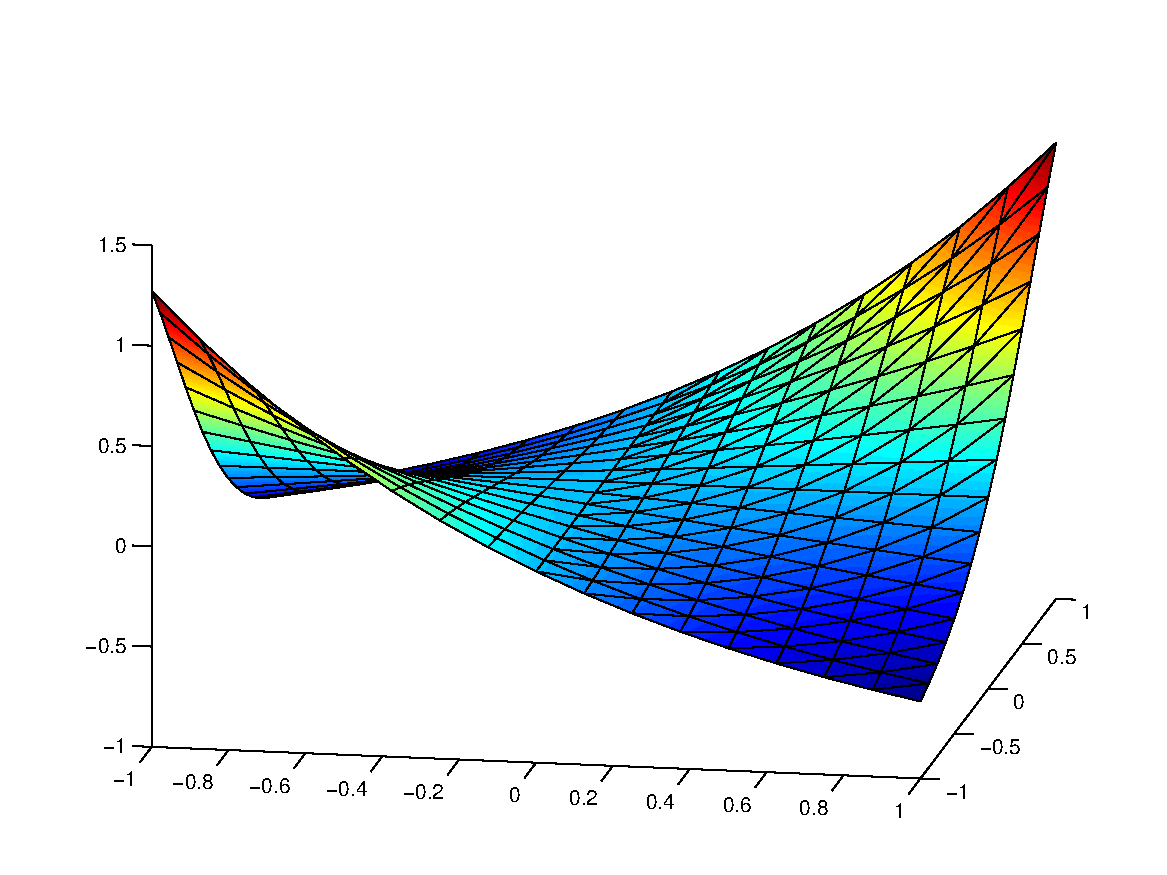
\includegraphics[height=0.27\textheight]{plots/poissonHybrid/phicubic16x16.pdf}\\
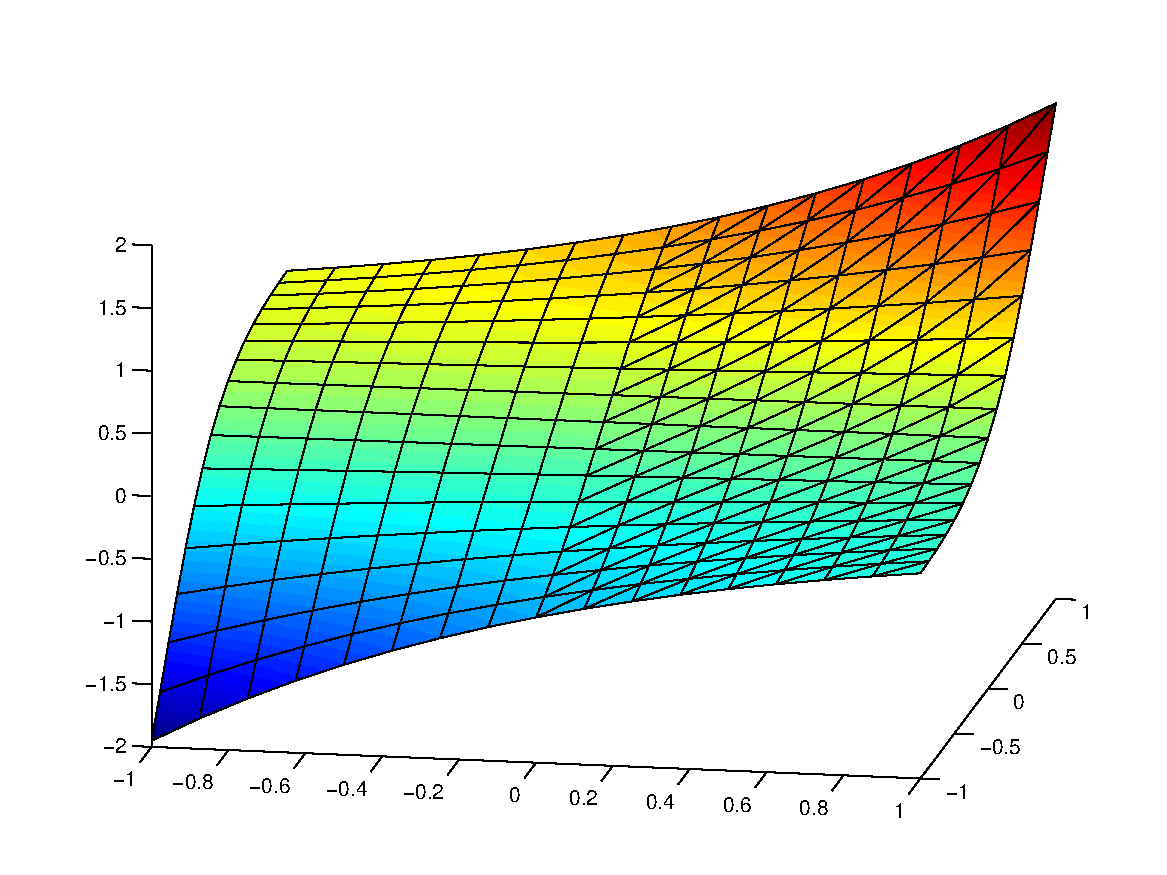
\includegraphics[height=0.27\textheight]{plots/poissonHybrid/psi1cubic16x16.pdf}\\
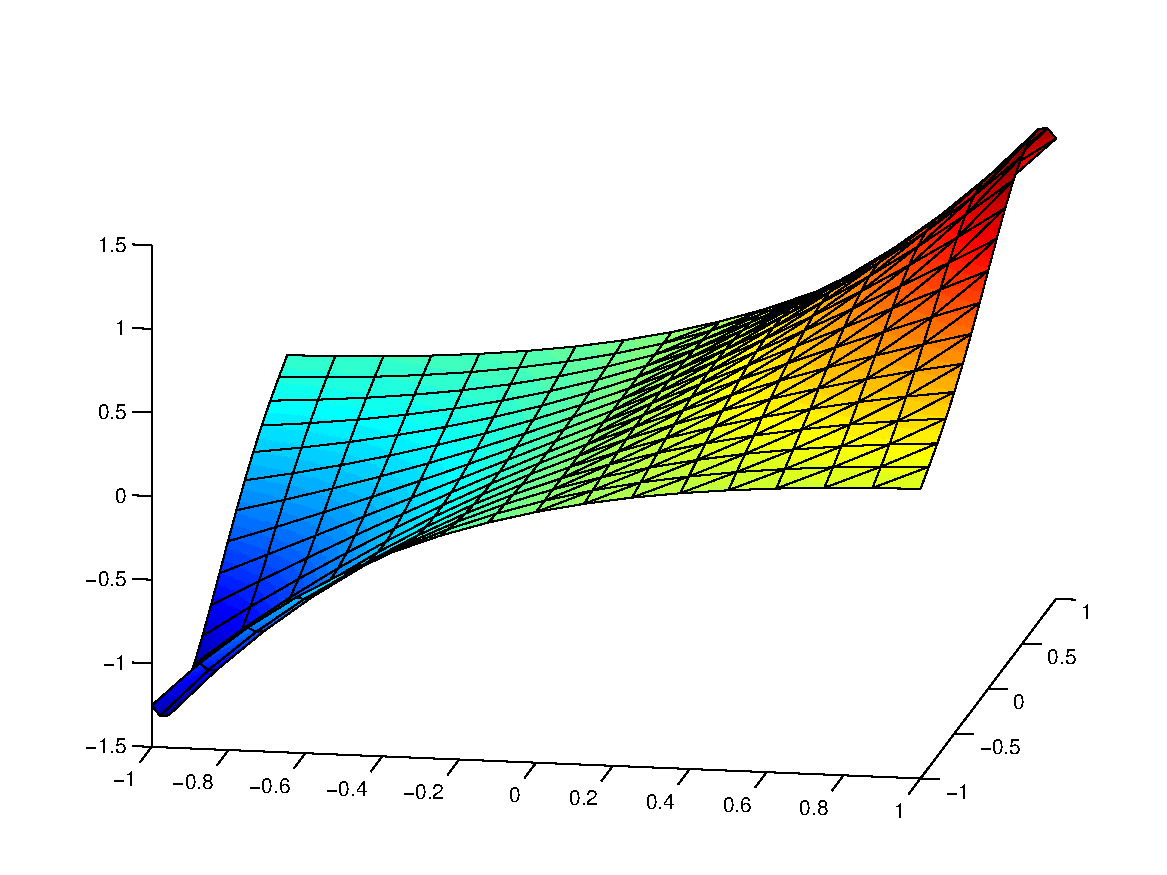
\includegraphics[height=0.27\textheight]{plots/poissonHybrid/psi2cubic16x16.pdf}
\caption{Solution of Poisson with quads and triangles (cubic elements, $16 \times 16$ mesh):
$\phi$ (top pane),
$\psi_{1}$ (middle pane)
$\psi_{2}$ (bottom pane).}
\label{NVR:fig:Poisson}
\end{center}\end{figure}

\begin{figure}[hbh]
\begin{center}
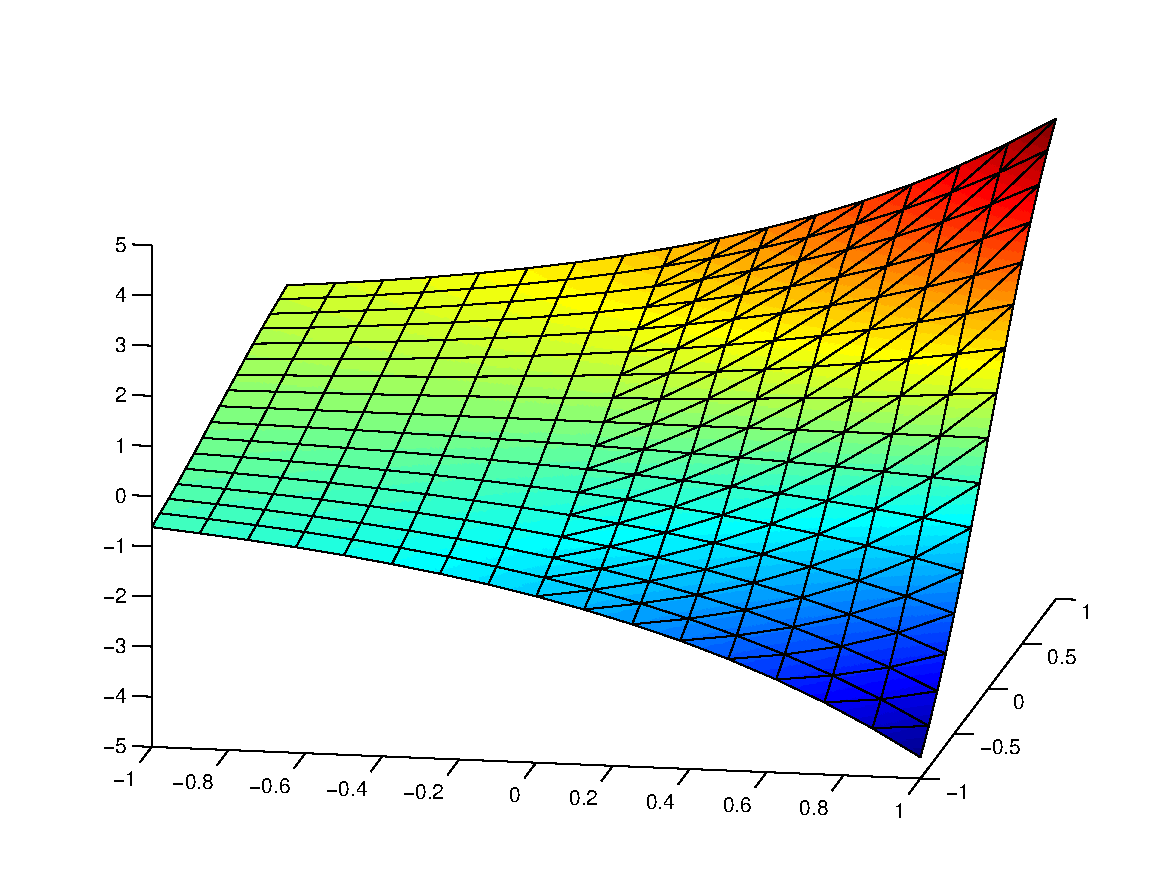
\includegraphics[height=0.27\textheight]{plots/stokesVVPHybrid/pressurecubic16x16.pdf}
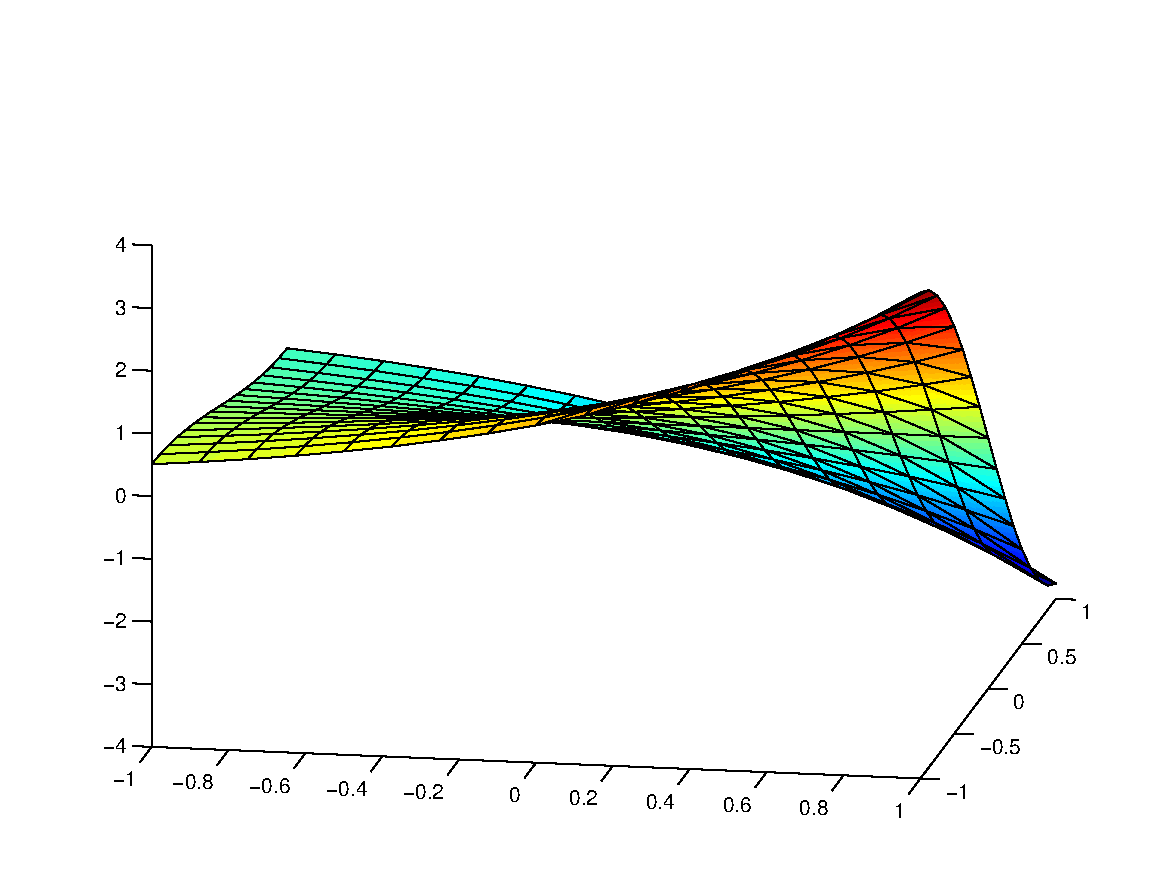
\includegraphics[height=0.27\textheight]{plots/stokesVVPHybrid/u1cubic16x16.pdf}
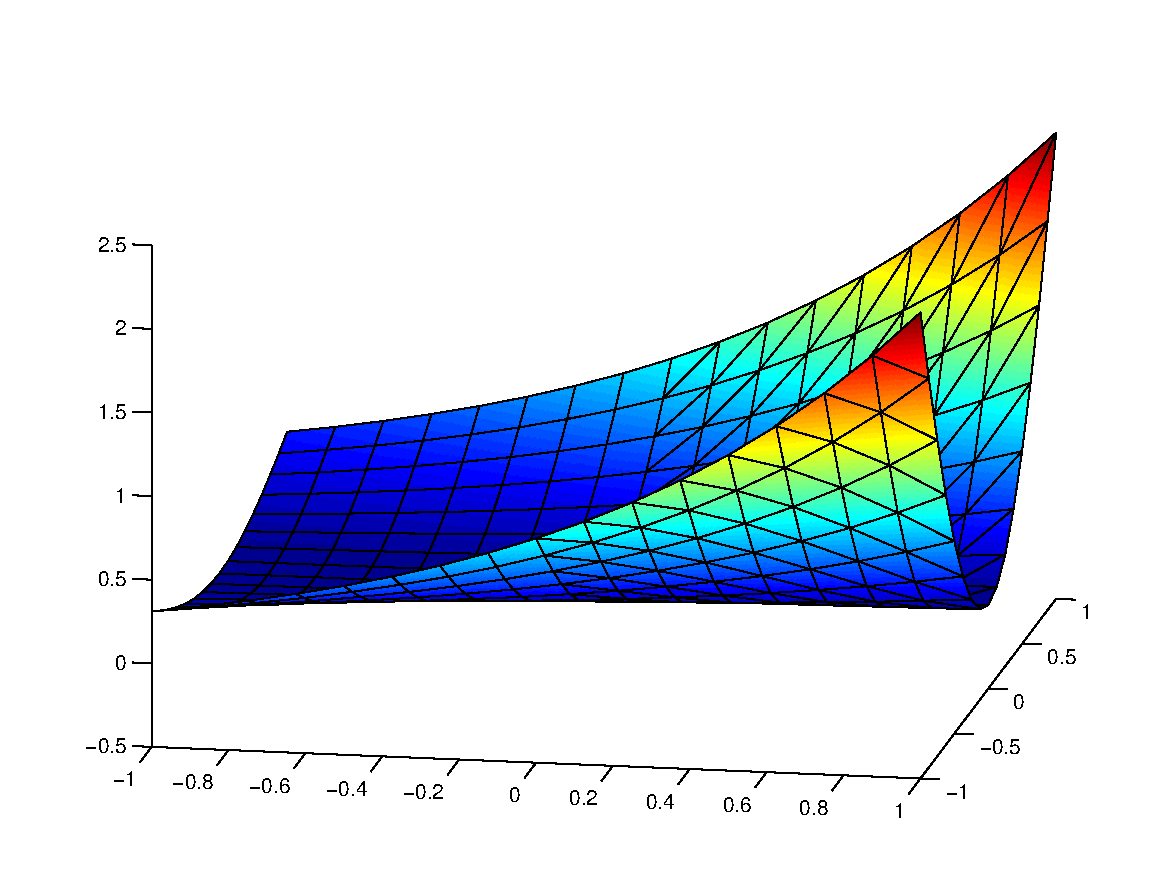
\includegraphics[height=0.27\textheight]{plots/stokesVVPHybrid/u2cubic16x16.pdf}
\caption{Solution of Stokes (VVP) with quads and triangles (cubic elements, $16 \times 16$ mesh):
$P$ (top pane),
$u_{1}$ (middle pane),
$u_{2}$ (bottom pane).}
\label{NVR:fig:Stokes}
\end{center}\end{figure}
